%! suppress = SentenceEndWithCapital
%! suppress = IncorrectSectionNesting
%! suppress = EscapeUnderscore
%! suppress = Ellipsis
A principal fiber bundle (often called simply principal bundle) is a mathematical object that formalizes some of the
essential features of the Cartesian product $X \times G$ of a space $X$ with a group $G$. In other words, very
roughly speaking, a principal bundle is a fiber bundle whose typical fiber is a Lie group. \v

A common example of a principal bundle is the frame bundle of a vector bundle, which consists of all ordered bases of
the vector space attached to each point. The group $G$ in this case is the general linear group, which acts on the
right in the usual way: by changes of basis. Since there is no natural way to choose an ordered basis of a vector
space, a frame bundle lacks a canonical choice of identity cross section. \v

Principal bundles have important applications in topology and differential geometry. They have also found application
in physics where they form part of the foundational framework of gauge theories. Principal bundles are so immensely
important because they allow us to understand any fiber bundle with fiber $F$ on which a Lie group $G$ acts. These
are then called associated fiber bundles (usually called associated bundles), and will be discussed later on.

\section{Principal Bundles}

\bd [Principal Bundle]
Let $G$ be a Lie group. A smooth bundle $(E,\pi,M)$ is called a \textbf{principal bundle} (or sometimes
\textbf{principal $G$-bundle}) if $E$ is equipped with a free right $G$-action and:
\bse
\begin{tikzcd}  E \ar[d,"\pi"'] \\ M \end{tikzcd} \ \ \cong_{\mathrm{bdl}}
\begin{tikzcd} E \ar[d,"\rho"]\\ E/G \end{tikzcd}
\ese

where $\rho$ is the quotient map, defined by sending each $p\in E$ to its equivalence class (i.e.\ orbit) in the
orbit space $E/G$.
\ed

Observe that since the right action of $G$ on $E$ is, by definition, free, for each $p\in E$ we have that the fiber
is the whole group:
\bse
\preim_\rho(G_p) = G_p \cong_{\mathrm{diff}} G
\ese

\v

We said at beginning that, roughly speaking, a principal bundle is a bundle whose fiber at each point is a Lie group.
Note that the formal definition is that a principal bundle is a bundle which is isomorphic to a bundle whose fibers
are the orbits under the right action of $G$, which are themselves isomorphic to $G$ since the action is free. \v

A slight generalisation would be to consider smooth bundles $E\xrightarrow{\,\pi\,}M$ where $E$ is equipped with a
right $G$-action which is free and transitive on each fiber of $E\xrightarrow{\,\pi\,}M$. The isomorphism in our
definition enforces the fiber-wise transitivity since $G$ acts transitively on each $G_p$ by the definition of orbit.

\subsection{Principal Bundle Maps}

As usual once we have defined a new object we want to define maps between these objects and study their morphisms. \v

Recall that a bundle morphism (also called simply a bundle map) between two bundles $(E,\pi,M)$ and $(E',\pi',M')$ is
a pair of maps $(u,f)$ such that the diagram:
\bse
\begin{tikzcd}
E \ar[dd,"\pi"'] \ar[rr,"u"] && E' \ar[dd,"\pi'"]\\ &&\\ M\ar[rr,"f"] && M'
\end{tikzcd}
\ese

commutes, that is, $f\circ \pi = \pi' \circ u$. As usual, two smooth bundles $(E,\pi,M)$ and $(E',\pi',M')$ are
isomorphic if $u,f$ are diffeomorphisms. We want now to extend these concepts from bundles to principal bundles. The
extension is not automatic since we have to take care of the extra structure of the underlying group.

\bd [Principal Bundle Map]
Let $(P,\pi,M)$ be a principal $G$-bundle, let $(P',\pi',M')$ be a principal $G'$-bundle, and let $\rho\cl G \to G'$
be a Lie group homomorphism. A \textbf{principal bundle morphism} from $(P,\pi,M)$ to $ (P',\pi',M')$ is a pair of
smooth maps $(u,f)$ such that the diagram:
\bse
\begin{tikzcd}
P \ar[rr,"u"]&& P' \\ &&\\
P \ar[uu,"{}\racts G"] \ar[dd,"\pi"'] \ar[rr,"u"] && P'\ar[uu,"{}\racts'
G'"'] \ar[dd,"\pi'"]\\ &&\\
M\ar[rr,"f"] && M'
\end{tikzcd}
\ese

\vspace{10pt}

commutes, that is:
\bi{rCl}
\forall \, p\in P : (f\circ \pi)(p) & = & (\pi'\circ u)(p)\\[5pt]
\forall \, p\in P : \forall \, g \in G : \ u(p\racts g) & = & u(p)\racts' \rho(g)
\ei
\ed

Note that one can restrict this general definition to the case where the same group $G$ acts in both principal
bundles (i.e.\ $G=G'$). In this case there is no Lie group homomorphism $\rho\cl G \to G'$, and the elements of the
group $G$ can act in both total spaces $P$ and $P'$ as they are. In this case the commutativity of the diagram
translates to:
\bi{rCl}
\forall \, p\in P : (f\circ \pi)(p) & = & (\pi'\circ u)(p)\\[5pt]
\forall \, p\in P : \forall \, g \in G : \ u(p\racts g) & = & u(p)\racts' g
\ei

where we keep the symbol $\racts'$ because we may define a different action in the two principal bundles. \v

\bd [Principal Bundle Isomorphism/Diffeomorphism]
A principal bundle morphism between a principal $G$-bundle and a principal $G'$-bundle is an \textbf{isomorphism} (or
\textbf{diffeomorphism}) \textbf{of principal bundles} if it is also a bundle isomorphism and $\rho$ is a Lie group
isomorphism.
\ed

Similarly in the case where $G=G'$, a principal bundle morphism between two principal $G$-bundles is an
\textbf{isomorphism} (or \textbf{diffeomorphism}) \textbf{of principal bundles} if it is also a bundle isomorphism.

\bt[]
Let $(P,\pi,M)$ and $(P',\pi',M)$ be principal bundles over the same base manifold $M$. Then, any $u\cl P \to
P'$ such that $(u,\id_M)$ is a principal bundle morphism is necessarily a diffeomorphism.

\bse
\begin{tikzcd}
P \ar[rr,"u"]&& P' \\ &&\\
P \ar[uu,"\racts G"] \ar[ddr,"\pi"'] \ar[rr,"u"] && P'\ar[uu,"\racts' G"'] \ar[ddl,"\pi'"]\\ &&\\ &M&
\end{tikzcd}
\ese
\et

\bq
We already know that $u$ is smooth since $(u,\id_M)$ is assumed to be a principal bundle morphism. It remains to
check that $u$ is bijective and its inverse is also smooth.
\ben[label=\roman*)]
\item Let $p_1,p_2\in P$ be such that $u(p_1)=u(p_2)$. Then:
\bse
\pi(p_1) = \pi'(u(p_1)) = \pi'(u(p_2)) = \pi(p_2)
\ese

that is, $p_1$ and $p_2$ belong to the same fiber. As the action of $G$ on $P$ is fiber-wise transitive, there is a
unique $g\in G$ such that $p_1 = p_2\racts g$. Then:
\bse
u(p_1) = u(p_2\racts g) = u(p_2) \racts' g = u(p_1) \racts' g
\ese

so $g\in S_{u(p_1)}$, but since $\racts'$ is free, we have $g=e$ and thus:
\bse
p_1 = p_2\racts e = p_2
\ese

Therefore $u$ is injective.
\item Let $p' \in P'$. Choose some $p\in \preim_\pi(\pi'(p'))$. Then, we have:
\bse
\pi'(u(p)) = \pi(p) = \pi'(p')
\ese

so that $u(p)$ and $p'$ belong to the same fiber. Hence, there is a unique $g\in G$ such that $p' = u(p)\racts' g$.
We thus have:
\bse
p' = u(p)\racts' g = u(p\racts g)
\ese

and since $p\racts g\in P$, the map $u$ is surjective.
\een

Hence, $u$ is a diffeomorphism.
\eq

\bd [Trivial Principal Bundle]
A principal $G$-bundle $(P,\pi,M)$ is called \textbf{trivial} if it is isomorphic as a principal bundle to the
principal $G$-bundle $(M\times G,\pi_1,M)$ where $\pi_1$ is the projection onto the first component and the action is
defined as:
\bi{rrCl}
\racts' \cl & (M\times G) \times G & \to &M\times G\\ & ((p,g),g') & \mapsto & (p,g)\racts' g' \coloneqq (p,g\bullet g')
\ei
\ed

By the previous lemma, a principal $G$-bundle $(P,\pi,M)$ is trivial if there exists a smooth map $u\cl P\to M\times
G$ such that the following diagram commutes:

\bse
\begin{tikzcd}
P \ar[rr,"u"]&& M\times G \\ &&\\
P \ar[uu,"{}\racts G"] \ar[ddr,"\pi"'] \ar[rr,"u"] && M\times G\ar[uu,"{}\racts' G"'] \ar[ddl,"\pi_1"]\\ &&\\ & M &
\end{tikzcd}
\ese

\vspace{10pt}

The following result provides a necessary and sufficient criterion for when a principal bundle is trivial. Note that
while we have used the lower case letter $p$ almost exclusively to denote points of the base manifold $M$, in the
next proof we will use it to denote points of the total space $P$ instead.

\bt[]
A principal $G$-bundle $(P,\pi,M)$ is trivial if, and only if, there exists a smooth section $\sigma\in\Gamma(P)$,
that is, a smooth $\sigma \cl M \to P$ such that $\pi\circ \sigma = \id_M$.
\et

Let's prove that!
\bit
\item[$(\Rightarrow)$] Suppose that $(P,\pi,M)$ is trivial. Then there exists a diffeomorphism $u\cl P \to M\times G$
which make the following diagram commute:
\bse
\begin{tikzcd}
P && \\ &&\\
P \ar[uu,"{}\racts G"] \ar[ddr,"\pi"'] && M \ar[ll,"u^{-1}"'] \times G\ar[ddl,"\pi_1"]\\ &&\\ & M &
\end{tikzcd}
\ese

We can define:
\bi{rrCl}
\sigma \cl & M & \to & P\\ & m & \mapsto & u^{-1}(m,e)
\ei

where $e$ is the identity of $G$. Then $\sigma$ is smooth since it is the composition of $u^{-1}$ with the map
$p\mapsto (p,e)$, which are both smooth. We also have:
\bse
(\pi\circ\sigma)(pm=\pi( u^{-1}(m,e)) = \pi_1 (m,e) = m
\ese

for all $m\in M$, hence, $\pi\circ\sigma=\id_M$ and thus $\sigma\in \Gamma(P)$.

\item[$(\Leftarrow)$] Suppose that there exists a smooth section $\sigma\cl M\to P$. Let $p\in P$ and consider the
point $\sigma(\pi(p))\in P$. We have:
\bse
\pi(\sigma(\pi(p))) = \id_M(\pi(p)) =\pi(p)
\ese

\v

Hence, $\sigma(\pi(p))$ and $p$ belong to the same fiber, and thus there exists a unique group element in $G$ which
links the two points via $\racts$. Since this element depends on both $\sigma$ and $p$, let us denote it by
$\chi_\sigma(p)$. Then, $\chi_\sigma$ defines a function:
\bi{rrCl}
\chi_\sigma \cl & P & \to & G\\ & p & \mapsto & \chi_\sigma(p)
\ei

and we can write:
\bse
\forall \, p \in P : \ p = \sigma(\pi(p))\racts \chi_\sigma(p)
\ese

In particular, for any other $g\in G$ we have $p\racts g\in P$ and thus:
\bse
p\racts g = \sigma(\pi(p\racts g))\racts \chi_\sigma(p\racts g) = \sigma(\pi(p))\racts \chi_\sigma(p\racts g)
\ese

where the second equality follows from the fact that the fibers of $P$ are precisely the orbits under the action of
$G$. On the other hand, we can act on the right with an arbitrary $g\in G$ directly to obtain:
\bse
p\racts g = (\sigma(\pi(p))\racts \chi_\sigma(p))\racts g = \sigma(\pi(p)) \racts (\chi_\sigma(p)\bullet g)
\ese

Combining the last two equations yields:
\bse
\sigma(\pi(p))\racts \chi_\sigma(p\racts g) = \sigma(\pi(p))\racts (\chi_\sigma(p)\bullet g)
\ese

and hence:
\bse
\chi_\sigma(p\racts g) = (\chi_\sigma(p)\bullet g)
\ese

We can now define the map:
\bi{rrCl}
u_\sigma \cl & P & \to & M \times G\\ & p & \mapsto & (\pi(p),\chi_\sigma(p))
\ei

By our previous lemma, it suffices to show that $u_\sigma$ is a principal bundle map.

\bse
\begin{tikzcd}
P \ar[rr,"u_\sigma"]&& M\times G \\ &&\\
P \ar[uu,"{}\racts G"] \ar[ddr,"\pi"'] \ar[rr,"u_\sigma"] && M\times G\ar[uu,"{}\racts' G"'] \ar[ddl,"\pi_1"]\\ &&\\
& M &
\end{tikzcd}
\ese

By definition, we have:
\bse
(\pi_1\circ u_\sigma)(p) = \pi_1 (\pi(p),\chi_\sigma(p))=\pi(p)
\ese

for all $p\in P$, so the lower triangle commutes. Moreover, we have:
\bi{rCl}
u_\sigma(p\racts g) & = & (\pi(p\racts g),\chi_\sigma(p\racts g))\\[5pt]
& = & (\pi(p),\chi_\sigma(p)\bullet g))\\[5pt]
& = & (\pi(p),\chi_\sigma(p))\racts' g\\[5pt]
& = & u_\sigma(p)\racts' g
\ei

for all $p\in P$ and $g\in G$, so the upper square also commutes and hence, $(P,\pi,M)$ is a trivial bundle. \qedhere
\eit

\section{Associated Bundles}

An associated fiber bundle (often called simply associated bundle) is a fiber bundle which is associated (in a
precise sense) to a principal $G$-bundle. Associated bundles are related to their underlying principal bundles in a
way that models the transformation law for components under a change of basis.

\bd [Associated Bundle]
Let $(P,\pi,M)$ be a principal $G$-bundle and let $F$ be a smooth manifold equipped with a left $G$-action $\lacts$.
We define:
\ben[label=\roman*)]
\item $P_F \coloneqq (P\times F)/{\sim_G}$, where $\sim_G$ is the equivalence relation:
\bse
(p,f) \sim_G (p',f') \quad :\Leftrightarrow \quad \exists \, g\in G : \biggl\{ \ba{rcl} p' & = & p\racts g \\ f' & =
& g^{-1} \lacts f \ea
\ese

We denote the points of $P_F$ as $[p,f]$.
\item The map:
\bi{rrCl}
\pi_F\cl & P_F & \to & M\\ & [p,f] & \mapsto & \pi(p)
\ei

which is well-defined since, if $[p',f']=[p,f]$, then for some $g\in G$:
\bse
\pi_F([p',f']) = \pi_F([p\racts g,g^{-1} \lacts f]) \coloneqq \pi(p\racts g) = \pi(p) \eqqcolon \pi_F([p,f])
\ese
\een

The \textbf{associated bundle} (to $(P,\pi,M)$, $F$ and $\lacts$) is the bundle $(P_F,\pi_F, M)$.
\ed

\subsection{Associated Bundle Maps}

Once we have defined associated bundles, we define maps between them and study their morphisms.

\bd [Associated Bundle Map]
Let $(P_F,\pi_F,M)$ to $(Q_F,\pi'_F,N)$ be the associated bundles (with the same fiber $F$) of two principal
$G$-bundles $(P,\pi,M)$ and $(P',\pi',M')$. An \textbf{associated bundle map} between the associated bundles is a
bundle map $(\widetilde u, \widetilde h)$ between them such that for some $u$, the pair $(u,h)$ is a principal bundle
map between the underlying principal $G$-bundles, i.e.\ :
\bi{rCl}
\forall \, p\in P : (\widetilde h\circ \pi)(p) & = & (\pi'\circ u)(p)\\[5pt]
\forall \, p\in P : \forall \, g \in G : \ u(p\racts g) & = & u(p)\racts' g
\ei

and on top of that:
\bse
\forall \, [p,f] \in P_F : (h \circ \pi_F)([p,f]) = (\pi'_F \circ \widetilde u)([p,f])
\ese

where :
\bi{rCl}
\forall \, [p,f] \in P_F : \widetilde u([p,f]) & \coloneqq & [u(p),f]\\[5pt]
\forall \, m \in M : \widetilde h (m) & \coloneqq & h (m)
\ei

Equivalently, the following \textbf{two} diagrams both commute:
\bse
\begin{tikzcd}
P_F \ar[dd,"\pi_F"'] \ar[rr,"\widetilde u"] && P'_F\ar[dd,"\pi_F'"]\\ &&\\ M \ar[rr,"\widetilde h"] && M'
\end{tikzcd}
\qquad \quad
\begin{tikzcd}
P \ar[rr,"u"]&& P' \\ &&\\ P \ar[uu,"\racts G"] \ar[dd,"\pi"'] \ar[rr,"u"] && P'\ar[uu,"\racts' G"'] \ar[dd,"\pi'"]\\
&&\\ M \ar[rr,"h"]&& M'
\end{tikzcd}
\ese
\ed

Since $\forall \, m \in M : \widetilde h (m) \coloneqq h (m)$ this simply implies that $\widetilde h = h$. From now
on we will simply denote $(\widetilde u, \widetilde h)$ a $(\widetilde u, h) $.

\bd [Associated Bundle Isomorphism]
An associated bundle map $(\widetilde u,h)$ is an \textbf{associated bundle isomorphism} if $\widetilde u$ and $h$
are invertible and $ (\widetilde u^{-1},h^{-1})$ is also an associated bundle map.
\ed

Note that two associated $F$-fiber bundles may be isomorphic as bundles but not as associated bundles. In other
words, there may exist a bundle isomorphism between them, but there may not exist any bundle isomorphism between them
which can be written as in the definition for some principal bundle isomorphism between the underlying principal
bundles. \v

Recall that an $F$-fiber bundle $(E,\pi,M)$ is called trivial if there exists a bundle isomorphism:
\bse
\adjustbox{scale=0.8,center}{
\begin{tikzcd}[scale=0.5]
F \ar[rr] && E\ar[ddr,"\pi"]\ar[rr,"u"] && M\times F \ar[ddl,"\pi_1"]\\ &&&&\\ &&& M &
\end{tikzcd}}
\ese

\v

while a principal $G$-bundle is called trivial if there exists a principal bundle isomorphism:
\bse
\adjustbox{scale=0.8,center}{
\begin{tikzcd}
P \ar[rr,"u"]&& M\times G \\ &&\\
P \ar[uu,"\racts G"] \ar[ddr,"\pi"'] \ar[rr,"u"] && M\times G\ar[uu,"\racts' G"'] \ar[ddl,"\pi_1"]\\ &&\\ & M &
\end{tikzcd}}
\ese

\v

\bd [Trivial Associated Bundle]
An associated bundle $(P_F,\pi_F,M)$ is called \textbf{trivial} if the underlying principal $G$-bundle $(P,\pi,M)$ is
trivial.
\ed

\bt[]
A trivial associated bundle is a trivial fiber bundle.
\et

Note that the converse does not hold. An associated bundle can be trivial as a fiber bundle but not as an associated
bundle, i.e.\ the underlying principal fiber bundle need not be trivial simply because the associated bundle is
trivial as a fiber bundle.

\bd [$H$-Restriction / $G$-Extension]
Let $H$ be a closed Lie subgroup of $G$. Let $(P,\pi,M)$ be a principal $H$-bundle and $(P',\pi',M)$ a principal
$G$-bundle. If there exists a principal bundle map from $(P,\pi,M)$ to $(P', \pi',M)$, i.e.\ a smooth bundle map
which is equivariant with respect to the inclusion of $H$ into $G$, then $(P,\pi, M)$ is called an$H$
\textbf{-restriction} of $(P',\pi',M)$, while $(P',\pi',M)$ is called a $G$\textbf{-extension} of $(P,\pi,M)$.
\ed

\bt[]
Let $H$ be a closed Lie subgroup of $G$.
\ben[label=\roman*)]
\item Any principal $H$-bundle can be extended to a principal $G$-bundle.
\item A principal $G$-bundle $(P,\pi,M)$ can be restricted to a principal $H$-bundle if, and only if, the bundle
$(P/H,\pi',M)$ has a section.
\een
\et

\section{Application: Principal Frame Bundle}

On of the most important examples of a principal $G$-bundle is the so called ``principal frame bundle". Given its
importance we will study it as a separate application. We will begin simply by defining it as a principal $G$-bundle.
We will do that in steps, so it's clear what we're doing.

\subsubsection*{Frame Bundle}

Let $M$ be a smooth manifold. Consider the space:
\bse
L_p M \coloneqq \{(e_1,\ldots,e_{\dim M})\mid e_1,\ldots,e_{\dim M} \text{is a basis of }T_p M\}
\ese

In other words, $L_p M$ is simply the collection (as a tuple) of the vectors of a basis of $T_p M$. We know from
linear algebra that the bases of a vector space are related to each other by invertible linear transformations.
Hence, we have:
\bse
L_p M \cong_{\mathrm{vec}} \GL(\dim M,\R)
\ese

We define the frame bundle of $M$ in the similar way as the tangent bundle:
\bse
LM \coloneqq \dot{\bigcup}_{p\in M}L_p M
\ese

with the obvious projection map $\pi\cl LM \to M$ sending each basis $(e_1, \ldots,e_{\dim M})$ to the unique point
$p\in M$ such that $(e_1,\ldots,e_{\dim M})$ is a basis of $T_p M$. \v

By proceeding similarly to the case of the tangent bundle, we can equip $LM$ with a smooth structure inherited from
that of $M$. We then find:
\bse
\dim LM = \dim M + \dim T_p M = \dim M + (\dim M)^2
\ese

\subsubsection*{Principal Frame Bundle}

We would now like to make $LM \xrightarrow{\,\pi\,}M$ into a principal $G$-bundle. Let us remind ourselves some
things we mentioned earlier. \v

Recall that we defined the set of all invertible maps $\mathrm{Aut}(V) \coloneqq \{\phi \in \mathrm{End}(V) \mid \phi
\text{ is an isomorphism}\}$, and we further said that we can equip this set with matrix multiplication and show that
it is closed under the operation, hence, we turn it into a group that we call $GL(V)$. On top of that, we can show
that $GL(V)$ is actually a topological group, hence, a Lie group, so it can be used as the group of a principal
$G$-bundle. \v

Recall also that the elements $g$ of $GL(V)$ are actually ``one-one" tensors (i.e.\ $g \in T^1_1 V$) and that once we
pick a basis, and we switch to the matrix notation then we can denote them as $g^a_{\phantom{a}b}$. Then we usually
denote the group as $\GL(n,V)$ where $n$ indicates the number of basis vectors (which is of course the dimension of
the manifold) and V the same underlying space as before. \v

Hence, in our case, we use as a group $G$ the group $\GL(\dim M,\R)$. We define a right $\GL(\dim M,\R)$-action on
$LM$ by:
\bse
(e_1,\ldots,e_{\dim M}) \racts g \coloneqq (g^a_{\phantom{a}1}e_a,\ldots, g^a_{\phantom{a}\dim M}e_a)
\ese

\v

where $g^a_{\phantom{a}b}$ are the components of the automorphism (usually called endomorphism but the invertibility
is implied) $g\in \GL(\dim M, \R)$ with respect to the standard basis on $\R^n$. Note that if $(e_1,\ldots,e_{\dim
M})\in L_p M$, we must also have $(e_1,\ldots,e_{\dim M}) \racts g\in L_p M$, hence, we just defined a mathematically
proper way to talk about a change of basis (linear basis transformations). \v

This action is free since:
\bse
(e_1,\ldots,e_{\dim M}) \racts g =
(e_1,\ldots,e_{\dim M}) \Leftrightarrow (g^a_{\phantom{a}1}e_a,\ldots, g^a_{\phantom{a}\dim M}e_a)= (e_1,\ldots,e_{\dim M})
\ese

and hence, by linear independence, $g^a_{\phantom{a}b}=\delta^a_b$, so $g=\id_{\R^n}$. Note that since all bases of
each $T_p M$ are related by some $g\in \GL(\dim M,\R)$, $\racts$ is also fiber-wise transitive. \v

We now have to show that:
\bse
\begin{tikzcd}
LM \ar[d,"\pi"'] \\ M
\end{tikzcd}
\ \ \cong_{\mathrm{bdl}}
\begin{tikzcd}
LM \ar[d,"\rho"]\\ LM \big/ \GL(\dim M,\R)
\end{tikzcd}
\ese

\v

i.e.\ that there exist smooth maps $u$ and $f$ such that the diagram: \v
\bse
\begin{tikzcd}
LM \ar[rr,shift left,"u"] \ar[dd,"\pi"']&& LM \ar[ll,shift left, "u^{-1}"]\ar[dd,"\rho"]\\ &&\\
M \ar[rr,shift left,"f"]&& LM \big/ \GL(\dim M,\R)\ar[ll,shift left, "f^{-1}"]
\end{tikzcd}
\ese

\v

commutes. \v

We can simply choose $u=u^{-1}=\id_{LM}$, while we define $f$ as:
\bi{rrCl}
f \cl & M & \to & LM\big/ \GL(\dim M,\R)\\[2pt] & p & \mapsto & \GL(\dim M,\R)_{(e_1,\ldots,e_{\dim M})}
\ei

where $(e_1,\ldots,e_{\dim M})$ is some basis of $T_p M$, i.e.\ $(e_1, \ldots,e_{\dim M})\in \preim_\pi(\{p\})$. Note
that $f$ is well-defined since every basis of $T_p M$ gives rise to the same orbit in the orbit space $LM\big/\GL
(\dim M,\R)$. Moreover, it is injective since:
\bse
f(p)=f(p')\ \Leftrightarrow \ \GL(\dim M,\R)_{(e_1,\ldots,e_{\dim M})} = \GL (\dim M,\R)_{(e'_1,\ldots,e'_{\dim M})}
\ese

which is true only if $(e_1,\ldots,e_{\dim M})$ and $(e'_1,\ldots,e'_{\dim M})$ are basis of the same tangent space,
so $p=p'$. It is clearly surjective since every orbit in $LM\big/ \GL(\dim M,\R)$ is the orbit of some basis of some
tangent space $T_p M$ at some point $p\in M$. The inverse map is given explicitly by:
\bi{rrCl}
f^{-1} \cl & LM\big/ \GL(\dim M,\R) & \to & M \\[2pt]
& \GL(\dim M,\R)_{(e_1,\ldots,e_{\dim M})} & \mapsto & \pi((e_1,\ldots,e_{\dim M}))
\ei

Finally, we have:
\bse
(\rho\circ\id_{LM})(e_1,\ldots,e_{\dim M}) = \GL(\dim M,\R)_{(e_1,\ldots, e_{\dim M})} = (f\circ \pi)(e_1,\ldots, e_{\dim M})
\ese

and thus $LM\xrightarrow{\,\pi\,}M$ is a principal $G$-bundle, called the \emph{principal frame bundle} of $M$ or
simply frame bundle. \v

A note to the careful reader. As we have just done in the previous example, in the following we will sometimes simply
assume that certain maps are smooth, instead of rigorously proving it.

\subsubsection*{Associated Frame Bundle}

Up to that point we showed that the frame bundle $(LM,\pi,M)$ is a principal $\GL(d,\R)$-bundle, where $d=\dim M$,
with right $G$-action $\racts\cl LM \times G \to LM$ given by:
\bse
(e_1,\ldots,e_{d}) \racts g \coloneqq (g^a_{\phantom{a}1}e_a,\ldots,g^a_{\phantom{a}d}e_a)
\ese

Let $F \coloneqq \R^{d}$ (as a smooth manifold) and define a left action:
\bi{rrCl}
\lacts \cl & \GL(d,\R) \times \R^{d} & \to & \R^{d}\\ & (g,x) & \mapsto & g\lacts x
\ei

where:
\bse
(g\lacts x)^a \coloneqq g^a_{\phantom{a}b} x^b
\ese

\v

Then $(LM_{\R^d},\pi_{\R^d},\R^d)$ is the associated bundle. In fact, we have a bundle isomorphism:
\bse
\begin{tikzcd}
LM_{\R^d} \ar[dd,"\pi_{\R^d}"'] \ar[rr,"u"] && TM\ar[dd,"\pi"] \\ && \\ M \ar[rr,"\id_M"] && M
\end{tikzcd}
\ese

\vspace{10pt}

where $(TM,\pi,M)$ is the tangent bundle of $M$, and $u$ is defined as:
\bi{rcCl}
u \cl & LM_{\R^d} & \to & TM\\ \v & [(e_1,\ldots,e_d),x] & \mapsto & x^ae_a
\ei

The inverse map $u^{-1}\cl TM \to LM_{\R^d}$ works as follows. Given any $X\in TM$, pick any basis $(e_1,\ldots,e_d)$
of the tangent space at the point $\pi(X)\in M$, i.e.\ any element of $L_{\pi(X)}M$. Decompose $X$ as $x^a e_a$, with
each $x^a\in \R$, and define:
\bse
u^{-1}(X) \coloneqq [(e_1,\ldots,e_d),x]
\ese

\v

The map $u^{-1}$ is well-defined since, while the pair $((e_1,\ldots,e_d),x) \in LM\times \R^d$ clearly depends on
the choice of basis, the equivalence class :
\bse
[(e_1,\ldots,e_d),x]\in LM_{\R^d} \coloneqq (LM\times \R^d)/{\sim_G}
\ese

does not. It includes all pairs $((e_1,\ldots,e_d)\racts g,g^{-1}\lacts x)$ for every $g\in \GL(d,\R)$, i.e.\ every
choice of basis together with the ``right'' components $x\in \R^d$. \v

Even though the associated bundle $(LM_{\R^d},\pi_{\R^d},\R^d)$ is isomorphic to the tangent bundle $(TM,\pi,M)$,
note a subtle difference between the two. On the tangent bundle, the transformation law for a change of basis and the
related transformation law for components are \emph{deduced} from the definitions by undergraduate linear algebra. \v

On the other hand, the transformation laws on $LM_{\R^d}$ were \emph{chosen} by us in its definition. We chose the
Lie group $\GL(d,\R)$, the specific right action $\racts$ on $LM$, the space $\R^d$, and the specific left action on
$\R^d$. It just happens that, with these choices, the resulting associated bundle is isomorphic to the tangent bundle.
Of course, we have the freedom to make different choices and construct bundles which behave very differently from
$TM$. \v

For example, consider now the principal $\GL(d,\R)$-bundle $(LM,\pi,M)$ again, with the same right action as before,
however this time we define a different fiber:
\bse
F \coloneqq (\R^d)^{\times p}\times({\R^d}^*)^{\times q} \coloneqq \underbrace{\R^d\times\cdots\times\R^d}_{p
\text{ times}}\times \underbrace{{\R^d}^*\times\cdots\times{\R^d}^*}_{q \text{ times}}
\ese

with left $\GL(d,\R)$-action $\lacts\cl\GL(d,\R)\times F \to F$ given by:
\bse
(g\lacts f)^{a_1\cdots a_p}_{\phantom{a_1\cdots a_p}b_1\cdots b_q} \coloneqq g^{a_1}_{\phantom{a_1}\widetilde a_1}
\cdots g^{a_p}_{\phantom{a_p}\widetilde a_p} (g^{-1})^{\widetilde b_1}_{\phantom{b_1}b_1}\cdots (g^{-1})^{\widetilde
b_q}_{\phantom{b_q}b_q} \, f^{\widetilde a_1\cdots \widetilde a_p}_{\phantom{a_1\cdots a_p}\widetilde b_1\cdots
\widetilde b_q}
\ese

Then, the associated bundle $(LM_F,\pi_F,M)$ thus constructed is isomorphic to $(T^p_q M,\pi,M)$, the $(p,q)$-tensor
bundle on $M$. \v

Now for something new, consider the following.

\bd [Tensor Density]
Let $M$ be a smooth manifold and let $(LM,\pi,M)$ be its frame bundle, with right $\GL(d,\R)$-action as above. Let $F
\coloneqq (\R^d)^{\times p}\times({\R^d}^*)^{\times q}$ and define a left $\GL(d,\R)$-action on $F$ by:
\bse
(g\lacts f)^{a_1\cdots a_p}_{\phantom{a_1\cdots a_p}b_1\cdots b_q} \coloneqq (\det g^{-1})^\omega\,
g^{a_1}_{\phantom{a_1}\widetilde a_1} \cdots g^{a_p}_{\phantom{a_p}\widetilde a_p} (g^{-1})^{\widetilde
b_1}_{\phantom{b_1}b_1}\cdots (g^{-1})^{\widetilde b_q}_{\phantom{b_q}b_q}\, f^{\widetilde a_1\cdots \widetilde
a_p}_{\phantom{a_1\cdots a_p}\widetilde b_1\cdots \widetilde b_q}
\ese

\v

where $\omega\in \Z$. Then the associated bundle $(LM_F,\pi_F,M)$ is called the \textbf{$(p,q)$-tensor
 $\omega$-density bundle} on $M$, and its sections are called \textbf{$ (p,q)$-tensor densities of weight} $\omega$. \ed

Some special cases include the following:
\ben[label=\roman*)]
\item If $\omega = 0$, we recover the $(p,q)$-tensor bundle on $M$.
\item If $F=\R$ (i.e.\ $p=q=0$), the left action reduces to:
\bse
(g\lacts f) = (\det g^{-1})^\omega\, f
\ese

which is the transformation law for a \emph{scalar density of weight $\omega$}.
\item If $\GL(d,\R)$ is restricted in such a way that we always have $(\det g^{-1})=1$, then tensor densities are
indistinguishable from ordinary tensor fields.
\een

Recall that if $B$ is a bilinear form on a $K$-vector space $V$, the determinant of $B$ is not independent of the
choice of basis. Indeed, if $\{e_a\}$ and $\{e'_b \coloneqq g^a_{\phantom{a}b}e_a\}$ are both basis of $V$, where
$g\in \GL(\dim V,K)$, then:
\bse
(\det B)' = (\det g^{-1})^2\det B
\ese

\v

Once recast in the principal and associated bundle formalism, we find that the determinant of a bilinear form is a
scalar density of weight $2$. \v

As a final note, remember the theorem we stated in the previous section, that for a closed Lie subgroup $H$ of $G$:
\ben[label=\roman*)]
\item Any principal $H$-bundle can be extended to a principal $G$-bundle.
\item A principal $G$-bundle $(P,\pi,M)$ can be restricted to a principal $H$-bundle if, and only if, the bundle $
(P/H,\pi',M)$ has a section.
\een

Coming to our case:
\ben[label=\roman*)]
\item The bundle $(LM/\SO(d),\pi,M)$ always has a section, and since $\SO(d) $ is a closed Lie subgroup of $\GL(d,\R)
$, the frame bundle can be restricted to a principal $\SO(d)$-bundle. This is related to the fact that any manifold
can be equipped with a Riemannian metric.
\item The bundle $(LM/\SO(1,d-1),\pi,M)$ may or may not have a section. For example, the bundle $(LS^2/\SO(1,1),\pi,
S^2)$ does not admit any section, and hence, we cannot restrict $(LS^2/\SO(1, 1),\pi,S^2)$ to a principal $\SO(1,1)
$-bundle, even though $\SO(1,1)$ is a closed Lie subgroup of $\GL(2,\R)$. This is related to the fact that the
$2$-sphere cannot be equipped with a Lorentzian metric.
\een

This concludes our application of principle fibre bundles to the very useful case of principle frame bundles. Now we
switch to the concept of connections on principle fibre bundles.

\section{Connections On A Principal Bundle}

Before proceeding with this chapter we need to make a very important statement that makes connection with the
previous chapter called ``Extra Structures On Topological Manifolds'' where we introduced (among others) the concept
of ``connection" (or ``covariant derivative") on a differentiable topological manifold. We said back in the chapter
that: ``connection and covariant derivative are not actually the same thing. In elementary courses on differential
geometry the notions of connection and covariant derivative are often confused with one another and, sometimes, the
terms are even used as synonyms. This happens because one is not in a position to properly define these concepts
before introducing the so-called ``principal fiber bundles" that we will do in a later chapter". And we moved on by
using a ``naive" way to introduce the concept. \v

However, now we are in a position to properly define those terms. In reality what a connection really is, is just
additional structure on a principal bundle consisting of a ``smooth'' assignment of a particular vector space at each
point of the base manifold compatible with the right action of the Lie group on the principal bundle. Such an
assignment is, in fact, equivalent to a certain Lie-algebra-valued one-form on the principal bundle, as we will
discuss below. Later, we will see that a connection on a principal bundle induces a parallel transport map on the
principal bundle, which in turn induces a parallel transport map on any of its associated bundles. If the fibers of
the associated bundle carry a vector space structure, then the parallel transport can be used to define a covariant
derivative on the associated bundle. \v

Hence, the conceptual sequence ``connection, parallel transport, covariant derivative'' is in decreasing order of
generality, and it should be clear that treating these terms as synonyms will inevitably lead to confusion. We will
now discuss the first of these in some detail. \v

Let $(P,\pi,M)$ be a principal $G$-bundle. Recall that every element of $X_e \in T_e G$ gives rise to a left
invariant vector field on $G$ which we denoted by $X = j(X_e) = ({\ell_{g*}})_e (X_{e})$. At this point we will
change our notation a bit since we will invoke vectors from different space. Namely, we will denote the element $X_e$
as $A_e$ hence, $A_e \in T_e G$. \v

We now define for every point $p \in P$ a map $i_p$ as follows:
\bi{rrCl}
i_p\cl & T_e G & \to & T_p P\\ & A_e & \mapsto & X^{A_e}_p
\ei

where:
\bi{rrCl}
X^{A_e}_p \cl & \mathcal{C}^\infty(P) &\xrightarrow{\sim} & \R \\
& f & \mapsto & X^{A_e}_p (f) \coloneqq [f(p\racts \exp(tA_e))]'(0)
\ei

where the derivative is to be taken with respect to $t$. It can be shown that $i_p$ is actually a Lie algebra
homomorphism.

\bd [Vertical Subspace]
Let $(P,\pi,M)$ be a principal bundle and let $p\in P$. The \textbf{vertical subspace} at $p$ is the vector subspace of
$T_p P$ given by:
\bi{rCl}
V_p P & \coloneqq & \ker((\pi_*)_p)\\[5pt] & = & \{X_p\in T_p P \mid (\pi_*)_p(X_p)=0\}
\ei
\ed

\bt[]
For all $A_e \in T_e G$ and $p\in P$, we have $X^{A_e}_p\in V_p P$.
\et

\bq
Since the action of $G$ simply permutes the elements within each fiber, we have:
\bse
\pi(p) = \pi(p\racts \exp(tA_e))
\ese

for any $t$. Let $f\in \mathcal{C}^\infty(M)$ be arbitrary. Then:
\bi{rCl}
(\pi_*)_pX^{A_e}_p(f) & = & X^{A_e}_p(f\circ \pi)\\[5pt]
& = & [(f\circ \pi)(p\racts \exp(tA_e))]'(0)\\[5pt]
& = & [f(\pi(p))]'(0)\\[5pt]
& = & 0
\ei

since $f(\pi(p))$ is constant. Hence, $X^{A_e}_p \in V_p P$. Alternatively, one can also argue that $(\pi_*) _p
X^{A_e}_p$ is the tangent vector to a constant curve on $M$. \eq

In particular, the map:
\bse
i_p\cl T_e G\xrightarrow{\sim} V_p P
\ese

is now a bijection. \v

The idea of a connection is to make a choice of how to ``connect'' the individual points in ``neighbouring'' fibers
in a principal fiber bundle.

\bd [Horizontal Subspace]
Let $(P,\pi,M)$ be a principal bundle and let $p\in P$. A \textbf{horizontal subspace} at $p$ a vector subspace $H_p P$
of $T_p P$ which is complementary to $V_p P$,
i.e.\ :
\bi{rCl}
T_p P = H_p P \oplus V_p P
\ei
\ed

The choice of horizontal space at $p\in P$ is not unique. However, once a choice is made, there is a unique
decomposition of each $X_p\in T_p P$ as:
\bse
X_p=\hor(X_p)+\ver(X_p)
\ese

with $\hor(X_p)\in H_p P$ and $\ver(X_p)\in V_p P$.

\bd [Connection]
A \textbf{connection} on a principal $G$-bundle $(P,\pi,M)$ is a choice of horizontal space at each $p\in P$ such that:
\ben[label=\roman*)]
\item For all $g\in G$, $p\in P$ and $X_p\in H_p P$, we have:
\bse
(\racts g_*)_p X_p \in H_{p\racts g}P
\ese

where $(\racts g_*)_p$ is the push-forward of the map $(-\racts g)\cl P \to P$ and it is a bijection.
\item For every smooth vector field $X\in \Gamma(TP)$, the two summands in the unique decomposition:
\bse
X_p = \hor(X_p)+\ver(X_p)
\ese

at each $p\in P$, extend to smooth $\hor(X),\ver(X)\in\Gamma(TM)$.
\een
\ed

The definition formalizes the idea that the assignment of an $H_p P$ to each $p\in P$ should be ``smooth'' within
each fiber (i) as well as between different fibers (ii). \v

For each $X_p\in T_p P$, both $\hor(X_p)$ and $\ver(X_p)$ depend on the choice of $H_p P$.

\subsection{Connection One-Forms}

Technically, the choice of a horizontal subspace $H_p P$ at each $p\in P$ providing a connection is conveniently
encoded in the thus induced Lie-algebra-valued one-form:
\bi{rrCl}
\omega_p \cl & T_p P & \xrightarrow{\sim} & T_e G\\ & X_p & \mapsto & \omega_p(X_p) \coloneqq i_p^{-1}(\ver(X_p))
\ei

\bd [Connection One-Form]
The map $\omega\cl p\to \omega_p$ sending each $p\in P$ to the $T_e G$-valued one-form $\omega_p$ is called the
\textbf{connection one-form} with respect to the connection.
\ed

We have seen how to produce a one-form from a choice of horizontal spaces (i.e.\ a connection). The choice of
horizontal spaces can be recovered from $\omega$ by:
\bse
H_p P = \ker (\omega_p)
\ese
Of course, not every (Lie-algebra-valued) one-form on $P$ is such that $\ker (\omega_p)$ gives a connection on the
principal bundle. What we would now like to do is to study some crucial properties of $\omega$. We will then elevate
these properties to a definition of connection one-form absent a connection, so that we may re-define the notion of
connection in terms of a connection one-form.

\bt[]
For all $p\in P$, $g\in G$ and $A_{e} \in T_e G$, we have:
\bse
(\racts g_*)_p X^{A_e}_p = X^{ {({\Ad_{g^{-1}}}*)}_e {A_e}}_{p\racts g}
\ese
\et

\bq
Let $f\in \mathcal{C}^\infty(P)$ be arbitrary. We have:
\bi{rCl}
(\racts g_*)_p X^{A_e}_p (f) & = & X^{A_e}_p (f\circ (-\racts g))\\[5pt]
& = & [f(p \racts \exp(t{A_e})\racts g)]'(0)\\[5pt]
& = & [f(p \racts g \racts g^{-1}\racts \exp(t{A_e})\racts g)]'(0)\\[5pt]
& = & [f(p \racts g \racts (g^{-1}\bullet \exp(t{A_e})\bullet g)]'(0)\\[5pt]
& = & [f(p \racts g \racts \Ad_{g^{-1}}(\exp(t{A_e}))]'(0)\\[5pt]
& = & [f(p \racts g \racts \exp(t {({\Ad_{g^{-1}}}*)}_e {A_e})]'(0)\\[5pt]
& = & X^{ {({\Ad_{g^{-1}}}*)}_e {A_e}}_{p\racts g} (f)
\ei
which is what we wanted.
\eq

\bt[]
A connection one-form $\omega$ with respect to a connection satisfies:
\ben[label=\alph*)]
\item For all $p\in P$, we have $\omega_p(X^A_p)=A$, that is $\omega_p\circ i_p = \id_{T_e G}$.
\bse
\adjustbox{scale=1.3,center}{
\begin{tikzcd}
T_e G \ar[rr,"i_p"] \ar[ddrr,"\id_{T_e G}"']&& V_p P \ar[dd, "\omega_p|_{V_p P}\phantom{nn}"]\\ &&\\ && T_e G
\end{tikzcd}}
\ese

\item $((\racts g)^*\omega)|_p (X_p)= (\Ad_{g^{-1}})_*(\omega_p(X_p))$.
\bse
\adjustbox{scale=1.3,center}{
\begin{tikzcd}
T_p P \ar[rr,"\omega_p"] \ar[ddrr,"((\racts g)^*\omega)|_p "']&& T_e G \ar[dd,"(\Ad_{g^{-1}})_*"]\\ &&\\ && T_e G
\end{tikzcd}}
\ese
\item $\omega$ is a smooth one-form.
\een
\et

\bq
\ben[label=\alph*)]
\item Since $X^A_p\in V_p P$, by definition of $\omega$ we have:
\bse
\omega_p(X^A_p) \coloneqq i_p^{-1}(\ver(X^A_p))=i_p^{-1}(X^A_p)=A
\ese

\item First observe that the left hand side is linear in $X_p$. Consider the two cases:
\ben[label=b.\arabic*)]
\item Suppose that $X_p\in V_p P$. Then $X_p=X_p^A$ for some $A\in T_e G$. Hence:
\bi{rCl}
((\racts g)^*\omega)|_p (X^A_p) & = & \omega_{p\racts g}((\racts g)_*X^A_p)\\
& = & \omega_{p\racts g}\Bigl(X^{(\Ad_{g^{-1}})_*A}_{p\racts g}\Bigr)\\
& = & (\Ad_{g^{-1}})_*A\\
& = & (\Ad_{g^{-1}})_*(\omega_p(X^A_p))
\ei

\item Suppose now that $X_p\in H_p P=\ker(\omega_p)$. Then:
\begin{equation*}
((\racts g)^*\omega)|_p (X_p) = \omega_{p\racts g}((\racts g)_*X_p) = 0
\end{equation*}

since $(\racts g)_*X_p\in H_{p\racts g}P=\ker(\omega_{p\racts g})$.
\een

Let $X_p\in T_p P$. We have:
\bi{rCl}
((\racts g)^*\omega)|_p (X_p) & = & ((\racts g)^*\omega)|_p (\ver(X_p)+\hor (X_p)) \\
& = & ((\racts g)^*\omega)|_p (\ver(X_p)) +((\racts g)^*\omega)|_p (\hor (X_p)) \\
& = & (\Ad_{g^{-1}})_*(\omega_p(\ver(X_p))) + 0 \\
& = & (\Ad_{g^{-1}})_*(\omega_p(\ver(X_p))) +(\Ad_{g^{-1}})_*(\omega_p(\hor (X_p)))\\
& = & (\Ad_{g^{-1}})_*(\omega_p(\ver(X_p)+\hor(X_p)))\\
& = & (\Ad_{g^{-1}})_*(\omega_p(X_p))
\ei

\item We have $\omega=i^{-1}\circ\ver$ and both $i^{-1}$ and $\ver$ are smooth.\qedhere
\een
\eq

\section{Yang-Mills Fields \& Local Representations}

A note for physics. Yang–Mills fields lead to the Yang–Mills theory which is very important for mathematical physics,
since it is a gauge theory based on a special unitary group, or more generally any compact, reductive Lie algebra.
Yang–Mills theory seeks to describe the behavior of elementary particles using these non-abelian Lie groups and is at
the core of the unification of the electromagnetic force and weak forces as well as quantum chromodynamics, the
theory of the strong force. Thus, it forms the basis of our understanding of the Standard Model of particle physics. \v

Now let's develop the theory mathematically. \v

We have seen so far how to associate a connection one-form to a connection, i.e.\ a certain Lie-algebra-valued
one-form to a smooth choice of horizontal spaces on the principal bundle. We will now study how we can express this
connection one-form locally on the base manifold of the principal bundle. \v

Recall that a connection one-form on a principal bundle $(P,\pi,M)$ is a smooth Lie-algebra-valued one-form, i.e.\ a
smooth map:
\bse
\omega\cl \Gamma(TP) \xrightarrow{\sim} T_e G
\ese

which ``behaves like a one-form'', in the sense that it is $\R$-linear and satisfies the Leibniz rule, and such that,
in addition, for all $A\in T_e G$, $g\in G$ and $X\in \Gamma(TP)$, we have:
\ben[label=\roman*)]
\item $\omega(X^A)=A$.
\item $((\racts g)^*\omega)(X)=(\Ad_{g^{-1}})_*(\omega(X))$.
\een

If the pair $(u,f)$ is a principal bundle automorphism of $(P,\pi,M)$, i.e.\ if the diagram:

\vspace{10pt}

\bse
\adjustbox{scale=1.3,center}{
\begin{tikzcd}
P \ar[rr,"u"]&& P \\ &&\\
P\ar[rr,"u"] \ar[dd,"\pi"'] \ar[uu,"\racts G"] && P\ar[dd,"\pi"] \ar[uu,"\racts G"'] \\ && \\ M \ar[rr,"f"]&& M
\end{tikzcd}}
\ese

\vspace{10pt}

commutes, we should be able to pull a connection one-form $\omega$ on $P$ back to another connection one-form
$u^*\omega$ on $P$.

\vspace{10pt}

\bse
\adjustbox{scale=1.3,center}{
\begin{tikzcd}
\Gamma(TP)\ar[rr,"\omega"] && T_e G \\ && \\
\Gamma(TP) \ar[uu,"u"] \ar[rruu,"u^*\omega"']&&
\end{tikzcd}}
\ese

\vspace{10pt}

Recall that for a one-form $\omega\cl \Gamma(TN) \xrightarrow{\sim}\mathcal{C}^\infty(N)$, we defined:
\bi{rrCl}
\Phi^*(\omega)\cl & \Gamma(TM) & \xrightarrow{\sim} & \mathcal{C}^\infty(M)\\ & X & \mapsto & \omega(\Phi_*(X))\circ \phi
\ei

for any diffeomorphism $\phi\cl M \to N$. One might be worried about whether this and similar definitions apply to
Lie-algebra-valued one-forms but, in fact, they do. In our case, even though $\omega$ lands in $T_e G$, its domain is
still $\Gamma(TP)$ and if $u\cl P\to P$ is a diffeomorphism of $P$, then $u_*X\in \Gamma(TP)$ and so:
\bse
u^*\omega\cl X \mapsto (u^*\omega)(X) \coloneqq \omega(u_*(X))\circ u
\ese

is again a Lie-algebra-valued one-form. Note that we will no longer distinguish notationally between the push-forward
of tangent vectors and of vector fields. \v

In practice, e.g.\ for calculational purposes, one may wish to restrict attention to some open subset $U\se M$. Let
$\sigma\cl U\to P$ be a local section of $P$, i.e.\ $\pi\circ \sigma = \id_U$.

\vspace{10pt}

\bse
\adjustbox{scale=1.3,center}{
\begin{tikzcd}
P\\ \\ P\ar[dd,"\pi"']\ar[uu,"\racts G"]\\ \\ U\ar[uu,bend right=60,"\sigma"']
\end{tikzcd}}
\ese

\bd [Yang-Mills Field / Local Trivialisation / Local Representation]
Given a connection one-form $\omega$ on $P$, such a local section $\sigma$ induces:
\ben[label=\roman*)]
\item A \textbf{Yang-Mills field} $\omega^U\cl \Gamma(TU) \xrightarrow{\sim} T_e G$ given by:
\bse
\omega^U \coloneqq \sigma^* \omega
\ese

\item A \textbf{local trivialisation} of the principal bundle $P$, i.e.\ a map:
\bi{rrCl}
h\cl & U\times G & \to & P\\ & (m,g)& \mapsto & \sigma(m)\racts g
\ei

\item A \textbf{local representation} of $\omega$ on $U$ by:
\bse
h^* \omega \cl \Gamma(T(U\times G)) \xrightarrow{\sim} T_e G
\ese
\een
\ed

Note that, at each point $(m,g)\in U\times G$, we have:
\bse
T_{(m,g)}(U\times G) \cong_{\mathrm{Lie \, alg}} T_mU\oplus T_g G
\ese

Both the Yang-Mills field $\omega^U$ and the local representation $h^*\omega$ encode the information carried by
$\omega$ locally on $U$. Since $h^*\omega$ involves $U\times G$ while $\omega^U$ doesn't, one might guess that
$h^*\omega$ gives a more ``accurate'' picture of $\omega$ on $U$ than the Yang-Mills field. But in fact, this is not
the case. They both contain the same amount of local information about the connection one-form $\omega$.

\subsection{The Maurer-Cartan Form}

Th relation between the Yang-Mills field and the local representation is provided by the following result.

\bt[]
For all $v\in T_m U$ and $\gamma \in T_g G$, we have:
\bse
(h^*\omega)_{(m,g)}(v,\gamma) = (\Ad_{g^{-1}})_*(\omega^U(v))+\Xi_g(\gamma)
\ese

where $\Xi_g$ is the Maurer-Cartan form:
\bi{rrCl}
\Xi_g \cl & T_g G & \xrightarrow{\sim} & T_e G\\ & L^A_g &\mapsto & A.
\ei
\et

\vspace{10pt}

\fig{maurer_cartan}{0.35}

Note that we have represented a generic element of $T_g G$ as $L^A_g$. This is due to the following. Recall that the
left translation map $\ell_g\cl G \to G$ is a diffeomorphism of $G$. As such, its push-forward at any point is a
linear isomorphism. In particular, we have:
\bse
((\ell_g)_*)_e \cl T_e G \xrightarrow{\sim} T_g G
\ese

that is, the tangent space at any point $g\in G$ can be canonically identified with the tangent space at the identity.
Hence, we can write any element of $T_g G$ as:
\bse
L^A_g \coloneqq ((\ell_g)_*)_e (A)
\ese

for some $A\in T_e G$. \v

Let us consider some specific examples.

\be
Any chart $(U,x)$ of a smooth manifold $M$ induces a local section $\sigma\cl U\to LM$ of the frame bundle of $M$ by:
\bse
\sigma(m) \coloneqq \biggl(\tvb{x}{1}{m},\ldots,\tvb{x}{\dim M}{m\,} \biggr) \in L_mM
\ese

Since $\GL(\dim M,\R)$ can be identified with an open subset of $\R^{(\dim M)^2}$, we have:
\bse
T_e\GL(\dim M,\R)\cong_{\mathrm{Lie\, alg}} \R^{(\dim M)^2}
\ese

where $\R^{(\dim M)^2}$ is understood as the algebra of $\dim M \times \dim M$ square matrices, with bracket induced
by matrix multiplication. In fact, this holds for any open subset of a vector space, when considered as a smooth
manifold. A connection one-form:
\bse
\omega\cl \Gamma(LM)\xrightarrow{\sim}T_e\GL(\dim M,\R)
\ese

can thus be given in terms of $(\dim M)^2$ functions:
\bse
\omega^i_{\phantom{i}j}\cl \Gamma(LM)\xrightarrow{\sim}\R, \qquad 1\leq i,j \leq \dim M
\ese

The associated Yang-Mills field $\omega^U \coloneqq \sigma^*\omega$ is, at each point $m\in U$, a Lie-algebra-valued
one-form on the vector space $T_m U$. By using the coordinate induced basis and its dual basis, we can express $
(\omega^U)_m$ in terms of components as:
\bse
(\omega^U)_m=\omega^U_\mu(m)\,(\d x^\mu)_m
\ese

where $1\leq \mu \leq \dim M$ and:
\bse
\omega^U_\mu(m) \coloneqq (\omega^U)_m\biggl(\tvb{x}{\mu}{m}\biggr)
\ese

Since $(\omega^U)_m\cl T_m U\xrightarrow{\sim}T_e G$, we have $\omega^U_\mu\cl U \to T_e G$. Hence, by employing he
same isomorphism as above, we can identify each $\omega^U_\mu(m)$ with a square $\dim M \times \dim M$ matrix and
define the symbol:
\bse
\Gamma^i_{\phantom{i}j\mu} (m) \coloneqq (\omega^U(m))^i_{\phantom{i}j\mu} \coloneqq (\omega^U_\mu(m))^i_{\phantom{i}j}
\ese

usually referred to as the \emph{Christoffel symbol}. The middle term is just an alternative notation for the
right-most side. Note that, even though all three indices $i$, $j$, $\mu$ run from $1$ to $\dim M$, the numbers
$\Gamma^i_{\phantom{i}j\mu} (m)$ do not constitute the components of a $(1,2)$-tensor on $U$. Only the $\mu$ index
transforms as a one-form component index, i.e.\ :
\bse
((g\lacts \omega^U(m))^i_{\phantom{i}j})_\mu = (g^{-1})^{\nu}_{\phantom{\mu}}(\omega^U(m))^i_{\phantom{i}j_\nu}
\ese

for $g\in \GL(\dim M,\R)$, while the $i$, $j$ indices simply label different one-forms, $(\dim M)^2$ in total.
\ee

Note that the Maurer-Cartan form only depends on the Lie group (and its Lie algebra), not on the principal bundle $P$
or the restriction $U\se M$. In the following example, we will go through the explicit calculation of the
Maurer-Cartan form of the Lie group $\GL(d, \R)$.

\be
Let $(\GL^+(d,\R),x)$ be a chart on $\GL(d,\R)$, where $\GL^+(d,\R)$ denotes an open subset of $\GL(d,\R)$ containing
the identity $\id_{\R^d}$, and let $x^i_{\phantom{i}j}\cl \GL^+(d,\R)\to \R$ denote the corresponding coordinate
functions:

\bse
\adjustbox{scale=1.3,center}{
\begin{tikzcd}
\GL^+(d,\R) \ar[ddrr,"x^i_{\phantom{i}j}"']\ar[rr,"x"]&& x(\GL^+(d,\R))\se \R^{d^2} \ar[dd, "\proj^i_{\phantom{i}j}"]\\
&&\\ && \R
\end{tikzcd}}
\ese

\vspace{10pt}

so that $x^i_{\phantom{i}j}(g) \coloneqq g^i_{\phantom{i}j}$. Recall that the coordinate functions are smooth maps
on the chart domain, i.e.\ we have $x^i_{\phantom{i}j}\in \mathcal{C}^\infty (\GL^+(d,\R))$. Also recall that to each
$A\in T_{\id_{\R^d}}\GL(d,\R)$ there is associated a left-invariant vector field:
\bse
L^A\cl \mathcal{C}^\infty(\GL^+(d,\R))\xrightarrow{\sim} \mathcal{C}^\infty (\GL^+(d,\R))
\ese

which, at each point $g\in \GL(d,\R)$, is the tangent vector to the curve:
\bse
\gamma^A(t) \coloneqq g\bullet \exp(tA)
\ese

Consider the action of $L^A$ on the coordinate functions:
\bi{rCl}
(L^Ax^i_{\phantom{i}j})(g) & = & [x^i_{\phantom{i}j}(g\bullet \exp(tA))]'(0)\\
& = & [x^i_{\phantom{i}j}(g\bullet\e^{tA})]'(0)\\
& = & (g^i_{\phantom{i}k}(\e^{tA})^k_{\phantom{k}j})'(0)\\
& = & g^i_{\phantom{i}k}A^k_{\phantom{k}j}
\ei

where we have used the fact that for a matrix Lie group, the exponential map is just the ordinary exponential:
\bse
\exp(A) = \e^A \coloneqq \sum_{n=0}^\infty \frac{1}{n!}A^n
\ese

Hence, we can write:
\bse
L^A|_g = g^i_{\phantom{i}k}A^k_{\phantom{k}j} \tvb{x^i_{\phantom{i}j}}{}{g}
\ese

from which we can read-off the Maurer-Cartan form of $\GL(d,\R)$:
\bse
(\Xi_g)^i_{\phantom{i}j} \coloneqq (g^{-1})^i_{\phantom{i}k} (\d x^k_{\phantom{k}j})_g
\ese

Indeed, we can quickly check that:
\bi{rCl}
(\Xi_g)^i_{\phantom{i}j}(L^A)
& = & (g^{-1})^i_{\phantom{i}k} (\d x^k_{\phantom{k}j})_g\biggl(g^p_{\phantom{p}r}A^r_{\phantom{r}q}
\tvb{x^p_{\phantom{p}q}}{}{g\,}\biggr) \\
& = & (g^{-1})^i_{\phantom{i}k}g^p_{\phantom{p}r}A^r_{\phantom{r}q}\delta^k_p\delta^q_j\\
& = & (g^{-1})^i_{\phantom{i}p}g^p_{\phantom{p}r}A^r_{\phantom{r}j}\\
& = & \delta^i_r A^r_{\phantom{r}j}\\
& = & A^i_{\phantom{i}j}
\ei
\ee

Now let's move to another topic.

\subsection{The Gauge Map}

In physics, we are often prompted to write down a Yang-Mills field because we have local information about a
connection. We can then try to reconstruct the global connection by glueing the Yang-Mills fields on several open
subsets of our manifold.
\bse
\adjustbox{scale=1.3,center}{
\begin{tikzcd}
&P \ar[ddl,"\pi"'] \ar[ddr,"\pi"] &\\ &&\\ U_1 \ar[uur,bend left=80,"\sigma_1"]&& U_2 \ar[uul,bend right=80, "\sigma_2"']
\end{tikzcd}}
\ese

Suppose, for instance, that we have two open subsets $U_1,U_2\se M$ and consider the Yang-Mills fields associated to
two local connections $\sigma_1,\sigma_2$. If $\omega^{U_1}$ and $\omega^{U_2}$ are both local versions of a unique
connection one-form, then is $U_1\cap U_2\neq \varnothing$, the Yang-Mills fields $\omega^{U_1}$ and $\omega^{U_2}$
should satisfy some compatibility condition on $U_1\cap U_2$.

\bd [Gauge Map]
Within the above set-up, the \textbf{gauge map} is the map:
\bse
\Omega \cl U_1\cap U_2 \to G
\ese

where, for each $m\in U_1\cap U_2$, the Lie group element $\Omega(m)\in G$ satisfies:
\bse
\sigma_2(m) = \sigma_1(m)\racts \Omega(m)
\ese
\ed

Note that since the $G$-action $\racts$ on $P$ is free, for each $m$ there exists an unique $\Omega(m)$ satisfying the
above condition, and hence, the gauge map $\Omega$ is well-defined.

\bt[]
Under the above assumptions, we have:
\bse
(\omega^{U_2})_m = (\Ad_{\Omega^{-1}(m)})_*( \omega^{U_1})+(\Omega^*\Xi_g)_m
\ese
\et

At this point Consider again the frame bundle $LM$ of some manifold $M$. Let us evaluate explicitly the pull-back
along $\Omega$ of the Maurer-Cartan form. Since $\Xi_g\cl T_g G \to T_e G$ and $\Omega\cl U_1\cap U_2\to T_e G$, we
have $\Omega^*\Xi_g\cl T(U_1\cap U_2)\to T_e G$. Let $x$ be a chart map near the point $m\in U_1\cap U_2$. We have:
\bi{rCl}
((\Omega^*\Xi_g)_m)^i_{\phantom{i}j} \biggl(\tvb{x}{\mu}{m\,}\biggr)
& = & (\Xi_{\Omega(m)})^i_{\phantom{i}j} \biggl (\Omega_*\tvb{x}{\mu}{m\,}\biggr) \\
& = & (\Omega(m)^{-1})^i_{\phantom{i}k} (\d \widetilde x^k_{\phantom{k}j})_{\Omega(m)}\biggl(\Omega_*\tvb{x}{\mu}{m\,
}\biggr) \\
& = & (\Omega(m)^{-1})^i_{\phantom{i}k} \biggl(\Omega_*\tvb{x}{\mu}{m\, }\biggr) (\widetilde x^k_{\phantom{k}j}) \\
& = & (\Omega(m)^{-1})^i_{\phantom{i}k} \tvb{x}{\mu}{m} (\widetilde x^k_{\phantom{k}j}\circ \Omega) \\
& = & (\Omega(m)^{-1})^i_{\phantom{i}k} \tvb{x}{\mu}{m} (\Omega(m))^k_{\phantom{k}j}
\ei

hence, we can write:
\bi{rCl}
((\Omega^*\Xi_g)_m)^i_{\phantom{i}j} & = & (\Omega(m)^{-1})^i_{\phantom{i}k} \tvb{x}{\mu}{m}
(\Omega(m))^k_{\phantom{k}j} \d x^\mu \\ & \eqqcolon & (\bm{\Omega}^{-1}\d \bm{\Omega})^i_{\phantom{i}j}
\ei

Let us now compute the other summand. Recall that $\Ad_g$ is the map:
\bi{rrCl}
\Ad_g \cl & G & \to & G \\ & h & \mapsto & g\bullet h \bullet g^{-1}
\ei

and since $\Ad_g(e)=e$, the push-forward $((\Ad_g)_*)_e\cl T_e G \xrightarrow{\sim} T_e G$ is a linear endomorphism
of $T_e G$. Moreover, since here $G=\GL(d,\R)$ is a matrix Lie group, we have:
\bse
((\Ad_g)_*A)^i_{\phantom{i}j} = g^i_{\phantom{i}k}A^k_{\phantom{k}l}(g^{-1})^l_{\phantom{l}j}
\eqqcolon (\bm{gAg}^{-1})^i_{\phantom{i}j}
\ese

Hence, we have:
\bi{rCl}
(\Ad_{\Omega^{-1}(m)})_*( \omega^{U_1}) & = & (\Omega(m)^{-1})^i_{\phantom{i}k}(\omega^{U_1})_m)^k_{\phantom{k}l}
(\Omega(m))^l_{\phantom{l}j}
\ei

Altogether, we find that the transition rule for the Yang-Mills fields on the intersection of $U_1$ and $U_2$ is
given by:
\bse
(\omega^{U_2})^i_{\phantom{i}j\mu} = (\Omega^{-1})^i_{\phantom{i}k}
(\omega^{U_1})^k_{\phantom{k}l\mu}\Omega^l_{\phantom{l}j}+
(\Omega^{-1})^i_{\phantom{i}k}\partial_\mu (\Omega^{-1})^k_{\phantom{k}j}
\ese

As an application, consider the spacial case in which the sections $\sigma_1,\sigma_2$ are induced by coordinate
charts $(U_1,x)$ and $(U_2,y)$. Then we have:
\bi{rCl}
\Omega^i_{\phantom{i}j} & = & \frac{\partial y^i}{\partial x^j} \coloneqq \partial_j(y^i\circ x^{-1})\circ x\\
(\Omega^{-1})^i_{\phantom{i}j} & = & \frac{\partial x^i}{\partial y^j} \coloneqq \partial_j(x^i\circ y^{-1})\circ y
\ei

and hence:
\bse
(\omega^{U_2})^i_{\phantom{i}j\nu} = \frac{\partial y^\mu}{\partial x^\nu} \biggl( \frac{\partial x^i}{\partial y^k}
(\omega^{U_1})^k_{\phantom{k}l\mu} \frac{\partial y^l}{\partial x^j} + \frac{\partial x^i}{\partial y^k}
\frac{\partial^2 y^k}{\partial x^\mu\partial x^j} \biggr)
\ese

\v

You may recognise this as the transformation law for the Christoffel symbols from previous chapter.


\section{Parallel Transport}

We now come to the second term in the sequence ``connection, parallel transport, covariant derivative''. The idea of
parallel transport on a principal bundle hinges on that of horizontal lift of a curve on the base manifold, which is
a lifting to a curve on the principal bundle in the sense that the projection to the base manifold of this curve
gives the curve we started with. In particular, if the principal bundle is equipped with a connection, we would like
to impose some extra conditions on this lifting, so that it ``connects'' nearby fibers in a nice way. We will then
consider the same idea on an associated bundle and see how we can induce a derivative operator if the associated
bundle is a vector bundle.

\subsection{Horizontal Lifts To The Principal Bundle}

Let's define the horizontal lift to the principle bundle.

\bd [Horizontal Lift (Principle Bundle)]
Let $(P,\pi,M)$ be a principal $G$-bundle equipped with a connection and let $\gamma\cl[0,1]\to M$ be a curve on $M$.
The \textbf{horizontal lift of $\gamma$ through $p_0\in P$} is the unique curve:
\bse
\gamma^{\uparrow}\cl [0,1] \to P
\ese

with $\gamma^\uparrow(0)=p_0\in \preim_\pi(\{\gamma(0)\})$ satisfying:
\ben[label=\roman*)]
\item $\pi \circ \gamma^{\uparrow} = \gamma$.
\item $\forall \, \lambda\in [0,1] : \ \ver(X_{\gamma^{\uparrow}, \gamma^{\uparrow}(\lambda)})=0$.
\item $\forall \, \lambda\in [0,1] : \ \pi_*(X_{\gamma^{\uparrow}, \gamma^{\uparrow}(\lambda)})=X_{\gamma,\gamma (\lambda)}$.
\een
\ed

Intuitively, a horizontal lift of a curve $\gamma$ on $M$ is a curve $\gamma^\uparrow$ on $P$ such that each point
$\gamma^\uparrow(\lambda)\in P$ belongs to the fiber of $\gamma(\lambda)$ (condition i), the tangent vectors to the
curve $\gamma^\uparrow$ have no vertical component (condition ii), i.e.\ they lie entirely in the horizontal spaces
at each point, and finally the projection of the tangent vector to $\gamma^\uparrow$ at $\gamma^\uparrow(\lambda)$
coincides with the tangent vector to the curve $\gamma$ at $\pi (\gamma^\uparrow(\lambda))=\gamma(\lambda)$. \v

Note that the uniqueness in the above definition only stems from the choice of $p_0\in\preim_\pi(\{\gamma(0)\})$. A
curve on $M$ has several horizontal lifts to a curve on $P$, but there is only one such curve going through each
point $p_0\in\preim_\pi(\{\gamma(0)\})$. Clearly, different horizontal lifts cannot intersect each other. \v

Our strategy to write down an explicit expression for the horizontal lift through $p_0\in P$ of a curve $\gamma\cl
[0,1]\to M$ is to proceed in two steps:

\ben[label=\roman*)]
\item ``Generate'' the horizontal lift by starting from some arbitrary curve $\delta\cl [0,1]\to P$ such that
$\pi\circ \delta = \gamma$ by action of a suitable curve $g\cl (0,1)\to G$ so that:
\bse
\gamma^\uparrow(\lambda) = \delta(\lambda)\racts g(\lambda)
\ese

The suitable curve $g$ will be the solution to an ordinary differential equation with initial condition $g(0)=g_0$,
where $g_0$ is the unique element in $G$ such that:
\bse
\delta(0)\racts g_0 = p_0\in P
\ese

\item We will explicitly solve (locally) this differential equation for $g\cl [0,1]\to P$ by a path-ordered integral
over the local Yang-Mills field.
\een

We have the following result characterising the curve $g$ appearing above.

\bt[]
The (first order) ODE satisfied by the curve $g\cl[0,1]\to G$ is:
\bse
(\Ad_{g(\lambda)^{-1}})_*(\omega_{\delta(\lambda)}(X_{\delta,\delta(\lambda)}))+\Xi_{g(\lambda)}(X_{g,g(\lambda)}) = 0
\ese

with the initial condition $g(0)=g_0$.
\et

We also have this theorem.

\bt[]
If $G$ is a matrix group, then the above ODE takes the form:
\bse
g(\lambda)^{-1}(\omega_{\delta(\lambda)}(X_{\delta,\delta(\lambda)}))g(\lambda)+g(\lambda)^{-1}\dot{g}(\lambda)=0
\ese

where we denoted matrix multiplication by juxtaposition and $\dot g(\lambda) $ denotes the derivative with respect to
$\lambda$ of the matrix entries of $g$. Equivalently, by multiplying both sides on the left by $g(\lambda)$:
\bse
\dot{g}(\lambda) = -(\omega_{\delta(\lambda)}(X_{\delta,\delta(\lambda)}))g(\lambda)
\ese
\et

We won't prove any of those. \v

In order to further massage this ODE, let us consider a chart $(U,x)$ on the base manifold $M$, such that the image
of $\gamma$ is entirely contained in $U$. A local section $\sigma\cl U \to P$ induces:
\ben[label=\roman*)]
\item A Yang-Mills field $\omega^U$.
\item A curve on $P$ by $\delta \coloneqq \sigma \circ \gamma$
\een

In fact, since the only condition imposed on $\delta$ is that $\pi\circ \delta = \gamma$, choosing a such a curve
$\delta$ is equivalent to choosing a local section $\sigma$. Note that we have:
\bse
\sigma_*(X_{\gamma,\gamma(\lambda)}) = X_{\delta,\delta(\lambda)}
\ese

and hence:
\bi{rCl}
\omega_{\delta(\lambda)}(X_{\delta,\delta(\lambda)})
& = & \omega_{\delta (\lambda)}(\sigma_*(X_{\gamma,\gamma (\lambda)}))\\
& = & (\sigma^*\omega)_{\gamma(\lambda)}(X_{\gamma,\gamma(\lambda)})\\
& = & (\omega^U)_{\gamma(\lambda)}(X_{\gamma,\gamma(\lambda)})\\
& = & \omega^U_\mu(\gamma(\lambda))(\d x^\mu)_{\gamma(\lambda)} \biggl (X_{\gamma}^\nu(\gamma(\lambda))
\tvb{x}{\nu}{\gamma(\lambda)\,}\biggr)\\
& = & \omega^U_\mu(\gamma(\lambda))X_{\gamma}^\nu(\gamma(\lambda))(\d x^\mu)_{\gamma(\lambda)} \biggl
(\tvb{x}{\nu}{\gamma(\lambda)\,}\biggr)\\
& = & \omega^U_\mu(\gamma(\lambda))X_{\gamma}^\nu(\gamma(\lambda))\, \delta^\mu_\nu\\
& = & \omega^U_\mu(\gamma(\lambda))X_{\gamma}^\mu(\gamma(\lambda))
\ei

\v

Thus, in the special case of a matrix Lie group, the ODE reads:
\bse
\dot{g}(\lambda) = -\Gamma_\mu(\gamma(\lambda))\, \dot{\gamma}^\mu(\lambda)
\ese

where $\Gamma_\mu \coloneqq \omega^U_\mu$ and $\dot{\gamma}^\mu(\lambda) \coloneqq X^\mu_{\gamma}(\gamma(\lambda))$,
together with the initial condition $g(0)=g_0$.

\subsection{Solution Of The horizontal Lift ODE By A Path-Ordered Exponential}

As a first step towards the solution of our ODE, consider:
\bse
g(t) \coloneqq g_0 -\int_0^t \d \lambda \, \Gamma_\mu(\gamma(\lambda))\,\dot{\gamma}^\mu(\lambda)g(\lambda)
\ese

This doesn't seem to have brought us far since the function $g$ that we would like to determine appears again on the
right hand side. However, we can now iterate this definition to obtain:
\bi{rCl}
g(t)
& = & g_0 -\int_0^t \d \lambda_1 \, \Gamma_\mu(\gamma(\lambda_1)) \dot{\gamma}^\mu(\lambda_1) \biggl(g_0
-\int_0^{\lambda_1} \d \lambda_2 \, \Gamma_\nu(\gamma(\lambda_2)) \dot{\gamma}^\nu(\lambda_2) \biggr)\\
& = & g_0 -\int_0^t \d \lambda_1 \, \Gamma_\mu(\gamma(\lambda_1)) \dot{\gamma}^\mu(\lambda_1)g_0+\int_0^t \d
\lambda_1\int_0^{\lambda_1} \d \lambda_2 \, \Gamma_\mu(\gamma(\lambda_1)) \dot{\gamma}^\mu(\lambda_1)\Gamma_\nu
(\gamma(\lambda_2)) \dot{\gamma}^\nu(\lambda_2)g(\lambda_2)
\ei

Matters seem to only get worse, until one realises that the first integral no longer contains the unknown function
$g$. Hence, the above expression provides a ``first-order'' approximation to $g$. It is clear that we can get
higher-order approximations by iterating this process:
\bi{rCl}
g(t) & = & g_0-\int_0^t \d \lambda_1 \, \Gamma_\mu(\gamma(\lambda_1)) \dot{\gamma}^\mu(\lambda_1)g_0\\
& & \phantom{g_0}+ \int_0^t \d \lambda_1\int_0^{\lambda_1} \d \lambda_2\, \Gamma_\mu(\gamma(\lambda_1))
\dot{\gamma}^\mu(\lambda_1)\Gamma_\nu(\gamma(\lambda_2)) \dot{\gamma}^\nu (\lambda_2) g_0\\
& & \phantom{g_0\,}\ \vdots\\
& & \phantom{g_0}+ (-1)^{n} \int_0^t \d \lambda_1\int_0^{\lambda_1} \d \lambda_2\, \cdots
\int_0^{\lambda_{n-1}}\d\lambda_n\, \Gamma_\mu(\gamma(\lambda_1)) \dot{\gamma}^\mu(\lambda_1)\cdots \Gamma_\nu
(\gamma(\lambda_n)) \dot{\gamma}^\nu(\lambda_n) \, g(\lambda_n)
\ei

Note how the range of each integral depends on the integration variable of the previous integral. It would much nicer
if we could have the same range in each integral. In fact, there is a standard trick to achieve this. The region of
integration in the double integral is:
\begin{center}
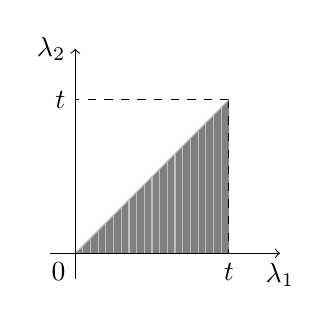
\begin{tikzpicture}[scale=0.65]
\draw (0,0) node[below left] {$0$};
\fill[gray] (0,0)--(3,0)--(3,3);
\draw[dashed] (3,3)--(3,0) node[below] {$t$};
\draw[dashed] (3,3)--(0,3) node[left] {$t$};
\foreach \i in {1,...,19} {
\draw[lightgray] (0.15*\i,0)--(0.15*\i,0.15*\i);};
\draw[lightgray] (0,0)--(3,3);
\draw[->] (-0.5,0)--(4,0) node[below] {$\lambda_1$};
\draw[->] (0,-0.5)--(0,4) node[left] {$\lambda_2$};
\end{tikzpicture}
\end{center}

and if the integrand $f(\lambda_1,\lambda_2)$ is invariant under the exchange $\lambda_1\leftrightarrow \lambda_2$,
we have:
\bse
\int_0^t \d \lambda_1\int_0^{\lambda_1} \d \lambda_2\, f(\lambda_1, \lambda_2)
= \frac{1}{2}\int_0^t \d \lambda_1\int_0^t \d \lambda_2\, f(\lambda_1,\lambda_2)
\ese

Generalising to $n$ dimensions, we have:
\bse
\int_0^t \d \lambda_1\,\cdots\int_0^{\lambda_{n-1}} \d \lambda_n\, f(\lambda_1,\ldots,\lambda_n)
= \frac{1}{n!}\int_0^t \d \lambda_1\,\cdots\int_0^t \d \lambda_n\, f(\lambda_1,\ldots,\lambda_n)
\ese

if $f$ is invariant under any permutation of its arguments. Moreover, since each term in our integrands only depends
on one integration variable at a time, we can use:
\bse
\int_0^t \d \lambda_1\,\cdots\int_0^{t} \d \lambda_n\, f_1(\lambda_1)\cdots f_n(\lambda_n) = \biggl(\int_0^t \d
\lambda_1\,f(\lambda_1)\biggr)\cdots\biggl(\int_0^t \d \lambda_n\, f(\lambda_n)\biggr)
\ese

so that, in our case, we would have:
\bi{rCl}
g(t) & = & \biggl(\,\sum_{n=0}^\infty \frac{(-1)^n}{n!}\biggl(\int_0^t \d \lambda \, \Gamma_\mu(\gamma(\lambda))
\dot{\gamma}^\mu(\lambda)\biggr)^{\negmedspace n\,} \biggr)g_0\\
& = & \exp\biggl(-\int_0^t \d \lambda \, \Gamma_\mu(\gamma(\lambda)) \dot{\gamma}^\mu(\lambda)\biggr) g_0
\ei

However, our integrands are Lie-algebra-valued (that is, matrix valued), and since the factors therein need not
commute, they are not invariant under permutations of the independent variables. Hence, the above formula doesn't
work. Instead, we write:
\bse
g(t)= \mathrm{P}\exp\biggl(-\int_0^t \d \lambda \, \Gamma_\mu(\gamma (\lambda))\dot{\gamma}^\mu(\lambda)\biggr) g_0
\ese

where the \emph{path-ordered exponential} $\mathrm{P}\exp$ is defined to yield the correct expression for $g(t)$. \v

Summarising, we have the following.

\bt[]
For a principal $G$-bundle $(P,\pi,M)$, where $G$ is a matrix Lie group, the horizontal lift of a curve $\gamma\cl
[0,1]\to U$ through $p_p\in \preim_\pi(\{U\})$, where $(U,x)$ is a chart on $M$, is given in terms of a local section
$\sigma\cl U \to P$ by the explicit expression:
\bse
\gamma^\uparrow(\lambda) = (\sigma\circ\gamma)(\lambda)\racts\biggl (\mathrm{P}\exp\biggl(-\int_0^\lambda \d
\widetilde\lambda \, \Gamma_\mu(\gamma(\widetilde\lambda))\dot{\gamma}^\mu (\widetilde\lambda)\biggr) g_0\biggr)
\ese
\et

\bd [Parallel Transport Map (Principle Bundle)]
Let $\gamma^\uparrow_p\cl[0,1]\to P$ be the horizontal lift through $p\in\preim_\pi(\{\gamma(0)\})$ of the curve
$\gamma\cl[0,1]\to M$. The \textbf{parallel transport map along $\gamma$} is the map:
\bi{rrCl}
T_\gamma \cl & \preim_\pi(\{\gamma(0)\}) & \to & \preim_\pi(\{\gamma(1)\}) \\ & p & \mapsto & \gamma^\uparrow_p(1)
\ei
\ed

The parallel transport is, in fact, a bijection between the fibers $\preim_\pi(\{\gamma(0)\})$ and $\preim_\pi
(\{\gamma(1)\})$. It is injective since there is a unique horizontal lift of $\gamma$ through each point
$p\in\preim_\pi(\{\gamma(0)\})$, and horizontal lifts through different points do not intersect. It is surjective
since for each $q\in \preim_\pi(\{\gamma(1)\})$ we can find a $p$ such that $q=\gamma^\uparrow_p(1)$ as follows. Let
$\widetilde p\in\preim_\pi(\{\gamma(0)\})$. Then $\gamma^\uparrow_{\widetilde p}(1)$ belongs to the same fiber as $q$
and hence, there exists a unique $g\in G$ such that $q = \gamma^\uparrow_{\widetilde p}(1) \racts g$. Recall that:
\bse
\gamma^\uparrow_{\widetilde p}(\lambda) = (\sigma\circ\gamma)(\lambda)\racts (\mathrm{P}\exp (\cdots ) g_0)
\ese

where $g_0$ is the unique $g_0\in G$ such that $\widetilde p = (\sigma\circ\gamma)(0)\racts g_0$. Define
$p\in\preim_\pi(\{\gamma(0)\})$ by:
\bse
p \coloneqq \widetilde p \racts g = (\sigma\circ\gamma)(0)\racts (g_0\bullet g)
\ese

Then we have:
\bi{rCl}
\gamma^\uparrow_{p}(1) & = & (\sigma\circ\gamma)(1)\racts (\mathrm{P}\exp (\cdots ) g_0\bullet g)\\
& = & (\sigma\circ\gamma)(1)\racts (\mathrm{P}\exp (\cdots ) g_0)\racts g\\
& = & \gamma^\uparrow_{\widetilde p}(1) \racts g\\
& = & q
\ei

\subsubsection*{Loops and holonomy groups}

Consider the case of loops, i.e.\ curves $\gamma\cl[0,1]\to M$ for which $\gamma(0)=\gamma(1)$. Fix some $p\in
\preim_\pi(\{\gamma(0)\})$. The condition that $\pi\circ\gamma_p^\uparrow=\gamma$ then implies that
$\gamma_p^\uparrow(0)$ and $\gamma_p^\uparrow(1)$ belong to the same fiber. Hence, there exists a unique $g_\gamma\in
G$ such that:
\bse
\gamma_p^\uparrow(1) = \gamma_p^\uparrow(0) \racts g_\gamma=p\racts g_\gamma
\ese

\bd [Holonomy Group]
Let $\omega$ be a connection one-form on the principal $G$-bundle $(P,\pi,M) $. Let $\gamma\cl[0,1]\to M$ be a loop
with base-point $a\in M$, i.e.\ $\gamma(0)=\gamma(1)=a$. The subgroup of $G$:
\bse
\Hol_a(\omega) \coloneqq \{g_\gamma \mid \gamma_p^\uparrow(1) =p\racts g_\gamma \text{ for some loop $\gamma$}\}
\ese

is called the \textbf{holonomy group} of $\omega$ on $P$ at the base-point $a$.
\ed

\subsection{Horizontal Lifts To The Associated Bundle}

Almost everything that we have done so far transfers with ease to an associated bundle via the following definition.

\bd [Horizontal Lift (Associated Bundle)]

Let $(P,\pi,M)$ be a principal $G$-bundle and $\omega$ a connection one-form on $P$. Let $(P_F,\pi_F,M)$ be an
associated fiber bundle of $P$ on whose typical fiber $F$ the Lie group $G$ acts on the left by $\lacts$. Let
$\gamma\cl [0,1]\to M$ be a curve on $M$ and let $\gamma^\uparrow_p$ be its horizontal lift to $P$ through $p\in
\preim_\pi(\{\gamma(0)\})$. Then the \textbf{horizontal lift} of $\gamma$ to the associated bundle $P_F$ through the
point $[p,f]\in P_F$ is the curve:
\bi{rrCl}
\gamma^{\negmedspace \stackrel{P_F}{\uparrow}}_{[p,f]} \cl & [0,1] & \to & P_F\\
& \lambda & \mapsto & [\gamma^\uparrow_p(\lambda),f]
\ei
\ed

For instance, we have the obvious parallel transport map.

\bd [Parallel Transport Map (Associated Bundle)]
The \textbf{parallel transport map} on the associated bundle is given by:
\bi{rrCl}
T^{P_F}_\gamma \cl & \preim_{\pi_F}(\{\gamma(0)\}) & \to & \preim_{\pi_F} (\{\gamma(1)\}) \\
& [p,f] & \mapsto & \gamma^{\negmedspace\stackrel{P_F}{\uparrow}}_{[p,f]}(1)
\ei
\ed

If $F$ is a vector space and $\lacts \cl G\times F \to F$ is fiber-wise linear, i.e.\ for each fixed $g\in G$, the
map $(g\lacts -)\cl F \to F$ is linear, then $(P_F,\pi_F,M)$ is called a \emph{vector bundle}. The basic idea of a
covariant derivative is as follows. Let $\sigma\cl U \to P_F$ be a local section of the associated bundle. We would
like to define the derivative of $\sigma$ at the point $m\in U\se M$ in the direction $X\in T_m M$. By definition,
there exists a curve $\gamma\cl(-\varepsilon,\varepsilon)\to M$ with $\gamma (0)=m$ such that $X=X_{\gamma,m}$. Then
for any $0\leq t <\varepsilon$, the points:
\bse
\gamma^{\negmedspace\stackrel{P_F}{\uparrow}}_{[\sigma(m),f]}(t) \qquad \text{and} \qquad \sigma(\gamma(t))
\ese

lie in the same fiber of $P_F$. \v

But since the fibers are vector spaces, we can write the differential quotient:
\bse
\frac{\sigma(\gamma(t))-\gamma^{\negmedspace\stackrel{P_F}{\uparrow}}_{[\sigma(m),f]}(t)}{t}
\ese

where the minus sign denotes the additive inverse in the vector space $\preim_{\pi_F}(\{\gamma(t)\})$ and hence
define the derivative of $\sigma$ at the point $m$ in the direction $X$, or the derivative of $\sigma$ along $\gamma$
at $\gamma(0)=m$, by:
\bse
\lim_{t\to 0} \frac{\sigma(\gamma(t)) - \gamma^{\negmedspace\stackrel{P_F}{\uparrow}}_{[\sigma(m),f]}(t)}{t}
\ese

\v

Of course, this makes sense as soon as we have a topology on the fibers). We will soon present a more abstract
approach. \v

Now let's move on to another topic.

\section{Covariant Exterior Derivative And Curvature}

Usually, in more elementary treatments of differential geometry curvature and torsion are mentioned together as
properties of a covariant derivative over the tangent or the frame bundle. Since we will soon define the notion of
curvature on a general principal bundle equipped with a connection, one might expect that there be a general
definition of torsion on a principal bundle with a connection. However, this is not the case. Torsion requires
additional structure beyond that induced by a connection. The reason why curvature and torsion are sometimes
presented together is that frame bundles are already equipped, in a canonical way, with the extra structure required
to define torsion. \v

Let's start by properly defining those terms.

\bd [Exterior Covariant Derivative]
Let $(P,\pi,M)$ be a principal $G$-bundle with connection one-form $\omega$. Let $\phi$ be a $k$-form (i.e.\ an
antisymmetric, $\mathcal{C}^\infty(P)$-multilinear map) with values in some module $V$. Then then \textbf{exterior
covariant derivative} of $\phi$ is:
\bi{rrCl}
\D\phi\cl & \Gamma(TP)^{\times (k+1)} & \to & V\\ & (X_1,\ldots,X_{k+1}) & \mapsto & \d \phi (\hor(X_1),\ldots,\hor(X_{k+1})).
\ei
\ed

\bd [Curvature]
Let $(P,\pi,M)$ be a principal $G$-bundle with connection one-form $\omega$. The \textbf{curvature} of the connection
one-form $\omega$ is the Lie-algebra-valued $2$-form on $P$:
\bse
\Omega\cl \Gamma(TP)\times \Gamma(TP) \to T_e G
\ese

defined by:
\bse
\Omega \coloneqq \D \omega
\ese
\ed

For calculational purposes, we would like to make this definition a bit more explicit.

\bt[]
Let $\omega$ be a connection one-form and $\Omega$ its curvature. Then:
\bse
\Omega = \d \omega + \omega \Wedge \omega
\ese

with the second term on the right hand side defined as:
\bse
(\omega\Wedge\omega )(X,Y) \coloneqq \llbracket\omega(X),\omega(Y) \rrbracket
\ese

where $X,Y\in \Gamma(TP)$ and the double bracket denotes the Lie bracket on $T_e G$.
\et

If $G$ is a matrix Lie group, and hence, $T_e G$ is an algebra of matrices of the same size as those of $G$, then we
can write:
\bse
\Omega^i_{\phantom{i}j} = \d \omega^i_{\phantom{i}j} + \omega^i_{\phantom{i}k}\wedge \omega^k_{\phantom{k}j}
\ese

\v

Let's prove this as an exercise. \v

Since $\Omega$ is $\mathcal{C}^\infty$-bilinear, it suffices to consider the following three cases:
\ben[label=\alph*)]
\item Suppose that $X,Y\in \Gamma(TP)$ are both vertical, that is, there exist $A,B\in T_e G$ such that $X=X^A$ and
$Y=X^B$. Then the left hand side of our equation reads:
\bi{rCl}
\Omega(X^A,X^B) & \coloneqq & \D\omega(X^A,X^B) \\ & = & \d \omega(\hor(X^A),\hor(X^B))\\ & = & \d \omega(0,0)\\ & = & 0
\ei

while the right hand side is:
\bi{rCl}
\d \omega(X^A,X^B) + (\omega\Wedge\omega )(X^A,X^B) & = & X^A(\omega(X^B)) -X^B(\omega(X^A))\\
&& {}-\omega([X^A,X^B])+ \left\llbracket \omega(X^A),\omega(X^B) \right\rrbracket\\
& = & X^A(B)-X^B(A)\\
&& {}-\omega(X^{\llbracket A,B\rrbracket} )+ \left\llbracket A, B\right\rrbracket\\
& = & -\left\llbracket A,B\right\rrbracket +\left\llbracket A, B\right\rrbracket\\
& = & 0
\ei

Note that we have used the fact that the map:
\bi{rrCl}
i\cl & T_e G & \to & \Gamma(TP)\\ & A \mapsto & X^A
\ei

is a Lie algebra homomorphism, and hence:

\bse
X^{\llbracket A,B\rrbracket}= i(\llbracket A,B\rrbracket) = [i(A),i(B)]=[X^A,X^B]
\ese

where the single square brackets denote the Lie bracket on $\Gamma(TP)$.

\item Suppose that $X,Y\in \Gamma(TP)$ are both horizontal. Then we have:
\bse
\Omega(X,Y) \coloneqq \D\omega(X,Y) = \d\omega(\hor(X),\hor(Y))=\d\omega(X,Y)
\ese

and:
\bse
(\omega\Wedge\omega )(X,Y) = \left\llbracket \omega(X),\omega(Y) \right\rrbracket = \left\llbracket 0, 0\right\rrbracket = 0
\ese

Hence, the equation holds in this case.

\item W.l.o.g suppose that $X\in \Gamma(TP)$ is horizontal while $Y=X^A\in\Gamma(TP)$ is vertical. Then the left hand
side is:
\bse
\Omega(X,X^A) \coloneqq \D \omega (X,X^A) = \d \omega(\hor(X),\hor(X^A)) = \d \omega(\hor(X),0) = 0
\ese

while the right hand side gives:
\bi{rCl}
\d \omega(X,X^A) + (\omega\Wedge\omega )(X,X^A) & = & X(\omega(X^A))-X^A (\omega(X))\\
&& {}-\omega([X,X^A])+ \left\llbracket \omega(X),\omega(X^A)\right\rrbracket\\
& = & X(A)-X^A(0)\\
&& {}-\omega(X^{\llbracket A,B\rrbracket} )+ \left\llbracket 0, A\right\rrbracket\\
& = & -\omega([X,X^A])\\
& = & 0
\ei

where the only non-trivial step, which is left as an exercise, is to show that if $X$ is horizontal and $Y$ is
vertical, then $[X,Y]$ is again horizontal.\qedhere
\een

\v

We would now like to relate the curvature on a principal bundle to (local) objects on the base manifold, just like we
have done for the connection one-form. Recall that a connection one-form on a principal $G$-bundle $(P,\pi,M)$ is a
$T_e G$-valued one-form $\omega$ on $P$. By using the notation $\Omega^1(P) \otimes T_e G$ for the collection (in
fact, bundle) of all $T_e G$-valued one-forms, we have $\omega\in\Omega^1(P) \otimes T_e G$. If $\sigma\in\Gamma(TU)$
is a local section on $M$, we defined the Yang-Mills field $\omega^U\in\Omega^1 (U)\otimes T_e G$ by pulling $\omega$
back along $\sigma$.

\bd [Yang-Mills Field Strength]
Let $(P,\pi,M)$ be a principal $G$-bundle and let $\Omega$ be the curvature associated to a connection one-form on
$P$. Let $\sigma\in\Gamma(TU)$ be a local section on $M$. Then, the two-form:
\bse
\Riem\equiv F \coloneqq \sigma^*\Omega \in \Omega^2(U)\otimes T_e G
\ese

is called the \textbf{Yang-Mills field strength}.
\ed

Observe that the equation $\Omega = \d \omega + \omega \Wedge \omega$ on $P$ immediately gives:
\bi{rCl}
\sigma^*\Omega & = & \sigma^*(\d \omega + \omega \Wedge \omega)\\
& = & \sigma^*(\d \omega) + \sigma^*(\omega \Wedge \omega)\\
& = & \d(\sigma^* \omega) + \sigma^*\omega \Wedge \sigma^*\omega
\ei

Since $\Riem$ is a two-form, we can write:
\bse
\Riem_{\mu\nu} = (\d \omega^U)_{\mu\nu} + \omega^U_{\mu} \Wedge \omega^U_{\nu}
\ese

In the case of a matrix Lie group, by writing $\Gamma^i_{\phantom{i}j\mu} \coloneqq (\omega^U)^i_{\phantom{i}j\mu}$,
we can further express this in components as:
\bse
\Riem^i_{\phantom{i}j\mu\nu} = \partial_\nu\Gamma^i_{\phantom{i}j\mu}-\partial_\mu\Gamma^i_{\phantom{i}j\nu} +
\Gamma^i_{\phantom{i}k\mu}\Gamma^k_{\phantom{k}j\nu}-\Gamma^i_{\phantom{i}k \nu}\Gamma^k_{\phantom{k}j\mu}
\ese

from which we immediately observe that $\Riem$ is symmetric in the last two indices, i.e.\ :
\bse
\Riem^i_{\phantom{i}j[\mu\nu]}=0
\ese

\bt[First Bianchi identity]
Let $\Omega$ be the curvature two-form associated to a connection one-form $\omega$ on a principal bundle. Then:
\bse
\D \Omega = 0
\ese
\et

Note that since $\Omega = \D\omega$, Bianchi's identity can be rewritten as $\D^2\Omega =0$. However, unlike the
exterior derivative $d$, the covariant exterior derivative does \emph{not} satisfy $\D^2 =0$ in general.

\subsection{Torsion}

\bd [Solder Form]
Let $(P,\pi,M)$ be a principal $G$-bundle and let $V$ be the representation space of a linear $(\dim M)$-dimensional
representation of the Lie group $G$. A \textbf{solder form} on $P$ is a one-form $\theta\in\Omega^1(P)\otimes V$ such
that:
\ben[label=(\roman*)]
\item $\forall \, X\in \Gamma(TP):\ \theta(\ver(X))=0$.
\item $\forall \,g\in G:\ g\lacts ((\racts g)^*\theta) = \theta$.
\item $TM$ and $P_V$ are isomorphic as associated bundles.
\een
\ed

A solder form provides an identification of $V$ with each tangent space of $M$.

\be
Consider the frame bundle $(LM,\pi,M)$ and define:
\bi{rrCl}
\theta \cl & \Gamma(T(LM)) & \to & \R^{\dim M}\\ & X & \mapsto & (u^{-1}_{\pi(X)}\circ \pi_*)(X)
\ei

where for each $e \coloneqq (e_1,\ldots,e_{\dim M}) \in LM$, $u_e$ is defined as:
\bi{rrCl}
u_e\cl & \R^{\dim M} & \xrightarrow{\sim} & T_{\pi(e)}M\\ & (x^1,\ldots,x^{\dim M}) & \mapsto & x^ie_i
\ei

To describe the inverse map $u_e^{-1}$ explicitly, note that to every frame $(e_1,\ldots,e_{\dim M}) \in LM$, there
exists a co-frame $(f^1,\ldots,f^{\dim M}) \in L^*M$ such that:
\bi{rrCl}
u_e^{-1}\cl & T_{\pi(e)}M & \xrightarrow{\sim} & \R^{\dim M}\\ & Z& \mapsto & (f^1(Z),\ldots,f^{\dim M}(Z))
\ei
\ee

\bd [Torsion]

Let $(P,\pi,M)$ be a principal $G$-bundle with connection one-form $\omega$ and let $\theta\in\Omega^1(P)\otimes V$
be a solder form on $P$. Then:
\bse
\Theta \coloneqq \D \theta \in\Omega^2(P)\otimes V
\ese

is the \textbf{torsion} of $\omega$ with respect to $\theta$.
\ed

You can now see that the ``extra structure'' required to define the torsion is a choice of solder form. The previous
example shows that there a canonical choice of such a form on any frame bundle. \v

We would like to have a similar formula for $\Theta$ as we had for $\Omega$. However, since $\Theta$ and $\theta$ are
both $V$-valued but $\omega$ is $T_e G$-valued, the term $\omega\Wedge\theta$ would be meaningless. What we have,
instead, is the following:
\bse
\Theta = \d \theta + \omega \halfWedge \theta
\ese

where the half-double wedge symbol intuitively indicates that we let $\omega$ act on $\theta$. More precisely, in the
case of a matrix Lie group, recalling that $\dim G = \dim T_e G = \dim V$, we have:
\bse
\Theta^i = \d \theta^i + \omega^i_{\phantom{i}k} \halfWedge \theta^k
\ese

\bt[Second Bianchi identity]
Let $\Theta$ be the torsion of a connection one-form $\omega$ with respect to a solder form $\theta$ on a principal
bundle. Then:
\bse
\D \Theta = \Omega \halfWedge \theta
\ese
\et

Like connection one-forms and curvatures two-forms, a torsion two-form $\Theta$ can also be pulled back to the base
manifold along a local section $\sigma$ as $T \coloneqq \sigma^*\Theta$. (In fact, \emph{this} is the torsion that
one typically meets in general relativity)

\section{Covariant Derivatives}

\subsection{Equivalence Of Local Sections And Equivariant Functions}

Recall that if $F$ is a vector space and $(P,\pi,M)$ a principal $G$-bundle equipped with a connection, we can use
the parallel transport on the associated bundle $(P_F,\pi_F,M)$ and the vector space structure of $F$ to define the
differential quotient of a local section $\sigma \cl U\to P_F$ along an integral curve of some tangent vector $X\in
TU$. This then allowed us to define the covariant derivative of $\sigma$ at the point $\pi(X)\in U$ in the direction
of $X\in TU$. \v

This approach to the concept of covariant derivative is very intuitive and geometric, but it is a disaster from a
technical point of view as it is quite difficult to implement. There is, in fact, a neater approach to covariant
differentiation, which will now discuss.

\bt[]
Let $(P,\pi,M)$ be a principal $G$-bundle and $(P_F,\pi_F,M)$ be an associated bundle. Let $(U,x)$ be a chart on $M$.
The local sections $\sigma\cl U \to P_F$ are in bijective correspondence with $G$-equivariant functions
$\phi\cl\preim_{\pi}(U)\subseteq P \to F$, where the $G$-equivariance condition is:
\bse
\forall \, g \in G : \forall \, p\in \preim_{\pi}(U) : \ \phi(g\racts p) = g^{-1}\lacts \phi(p)
\ese
\et

As an exercise let's try to prove this. \v

\ben[label=(\alph*)]
\item Let $\phi\preim_{\pi}(U) \to F$ be $G$-equivariant. Define:
\bi{rrCl}
\sigma_{\phi}\cl & U & \to & P_F\\ & m & \mapsto & [p,\phi(p)]
\ei

where $p$ is any point in $\preim_{\pi}(\{m\})$. First, we should check that $\sigma_{\phi}$ is well-defined. Let $p,
\widetilde p\in \preim_{\pi}(\{m\})$. Then, there exists a unique $g\in G$ such that $\widetilde p = p\racts g$.
Then, by the $G$-equivariance of $\phi$, we have:
\bse
[\widetilde p,\phi(\widetilde p)] = [p\racts g,\phi(p\racts g)] = [p\racts g,g^{-1}\lacts \phi(p)] = [p,\phi(p)]
\ese

and hence, $\sigma_{\phi}$ is well-defined. Moreover, since for all $g\in G$:
\bse
\pi_F([p,\phi(p)]) = \pi(p) =\pi(p\racts g)= \pi_F([p\racts g,g^{-1}\lacts \phi(p)])
\ese

we have $\pi_F\circ\sigma_{\phi}=\id_U$ and thus, $\sigma_{\phi}$ is a local section.

\item Let $\sigma\cl U\to P_F$ be a local section. Define:
\bi{rrCl}
\phi_{\sigma}\cl & \preim_{\pi}(U) & \to & F\\ & p & \mapsto & i^{-1}_p(\sigma(\pi(p)))
\ei

where $i^{-1}_p$ is the inverse of the map:
\bi{rrCl}
i_p\cl & F & \to & \preim_{\pi_F}(\{\pi(p)\})\subseteq P_F\\ & f & \mapsto & [p,f]
\ei

Observe that, for all $g\in G$, we have:
\bse
i_p(f) \coloneqq [p,f]=[p\racts g,g^{-1}\lacts f] \eqqcolon i_{p\racts g} (g^{-1}\lacts f)
\ese

Let us now show that $\phi_{\sigma}$ is $G$-equivariant. We have:
\bi{rCl}
\phi_{\sigma}(p\racts g) & = & i^{-1}_{p\racts g}(\sigma(\pi(p\racts g)))\\
& = & i^{-1}_{p\racts g}(\sigma(\pi(p)))\\
& = & i^{-1}_{p\racts g}(i_p(\phi_{\sigma}(p)))\\
& = & i^{-1}_{p\racts g}(i_{p\racts g}(g^{-1}\lacts\phi_{\sigma}(p)))\\
& = & g^{-1}\lacts\phi_{\sigma}(p)
\ei

which is what we wanted.

\item We now show that these constructions are the inverses of each other, i.e.\ :
\bse
\sigma_{\phi_{\sigma}} = \sigma, \qquad \quad \phi_{\sigma_{\phi}} = \phi
\ese

Let $m\in U$. Then, we have:
\bi{rCl}
\sigma_{\phi_{\sigma}}(m) & = & [p,\phi_{\sigma}(p)]\\
& = & [p,i^{-1}_p(\sigma(\pi(p)))]\\
& = & i_p(i^{-1}_p(\sigma(\pi(p))))\\
& = & \sigma(\pi(p))\\
& = & \sigma(m)
\ei

and hence, $\sigma_{\phi_{\sigma}} = \sigma$. Now let $p\in \preim_{\pi}(U)$.  Then, we have:
\bi{rCl}
\phi_{\sigma_{\phi}}(p) & = & i^{-1}_p(\sigma_{\phi}(\pi(p)))\\
& = & i^{-1}_p([p,\phi(p)])\\
& = & i^{-1}_p(i_p(\phi(p)))\\
& = & \phi(p)
\ei

and hence, $\phi_{\sigma_{\phi}} = \phi$. \qedhere
\een

\subsection{Linear Actions On Associated Vector Fiber Bundles}

We now specialise to the case where $F$ is a vector space, and hence, we can require the left action $G\!\lacts \cl
F\xrightarrow{\sim} F$ to be linear.

\bt[]

Let $(P,\pi,M)$ be a principal $G$-bundle, and let $(P_F,\pi_F,M)$ be an associated bundle, where $G$ is a matrix Lie
group, $F$ is a vector space, and the left $G$-action on $F$ is linear. Let $\phi\cl P\to F$ be $G$-equivariant. Then:
\bse
\phi(p\racts \exp(At)) = \exp(-At)\lacts \phi(p)
\ese

where $p\in P$ and $A\in T_e G$.
\et

\bt[]
With the same assumptions as above, let $A\in T_e G$ and let $\omega$ be a connection one-form on $(P,\pi,M)$. Then:
\bse
\d \phi(X^A) + \omega(X^A)\lacts \phi = 0
\ese
\et

Let's prove this.

\bq
Since $\phi$ is $G$-equivariant, by applying the previous proposition, we have:
\bse
\phi(p\racts \exp(At)) = \exp(-At)\lacts \phi(p)
\ese

for any $p\in P$. Hence, differentiating with respect to $t$ yields:
\bi{rCl}
(\phi(p\racts \exp(At)))'(0) & = &
(\exp(-At)\lacts \phi(p))'(0)\\ \d_p\phi(X^A) & = & -A \lacts \phi(p)\\ \d_p\phi(X^A) & = & -\omega(X^A) \lacts \phi(p)
\ei

for all $p\in P$ and hence, the claim holds.
\eq

\subsection{Construction Of The Covariant Derivative}

We now wish to construct a covariant derivative, i.e.\ an ``operator'' $\nabla$ such that for any local section
$\sigma \cl U \subseteq M \to P_F$ and any $X\in T_m U$ with $m\in U$, we have that $\nabla_X \sigma$ is again a
local section $U\to P_F$ and:
\ben[label=\roman*)]
\item $\nabla_{fX+Y}\sigma = f\nabla_{X}\sigma+\nabla_{Y}\sigma$.
\item $\nabla_X(\sigma+\tau) = \nabla_X\sigma+\nabla_X\tau$.
\item $\nabla_X f\sigma = X(f)\sigma+f\nabla_X\sigma$.
\een

for any sections $\sigma,\tau\cl U\to P_F$, any $f\in \mathcal{C}^{\infty} (U)$, and any $X,Y\in T_m U$. \v

These (together with $\nabla_X f \coloneqq X(f)$) are usually presented as the defining properties of the covariant
derivative in more elementary treatments. \v

Recall that functions are a special case of forms, namely the $0$-forms, and hence, the exterior covariant derivative
a function $\phi\cl P\to F$ is:
\bse
\D\phi \coloneqq \d \phi \circ \hor
\ese

We now have the following theorem.

\bt[]
Let $\phi\cl P\to F$ be $G$-equivariant and let $X\in T_p P$. Then:
\bse
\D\phi(X) = \d\phi(X)+\omega(X)\lacts \phi
\ese
\et

\bq
\ben[label=(\alph*)]
\item Suppose that $X$ is vertical, that is, $X=X^A$ for some $A\in T_e G$. Then:
\bse
\D\phi(X) = \d\phi(\hor(X))=0
\ese

and:
\bse
\d\phi(X^A)+\omega(X^A)\lacts \phi = 0
\ese

by the previous corollary.
\item Suppose that $X$ is horizontal. Then:
\bse
\D\phi(X)=\d\phi(X)
\ese

and $\omega(X)=0$, so that we have:
\bse
\D\phi(X) = \d\phi(X)+\omega(X)\lacts \phi\qedhere
\ese
\een
\eq

Hence, it is clear from this proposition that $\D\phi(X)$, which we can also write as $\D_X\phi$, is
$\mathcal{C}^{\infty}(P)$-linear in the $X$-slot, additive in the $\phi$-slot and satisfies property iii) above.
However, it also clearly \emph{not} a covariant derivative since $X\in TP$ rather than $X\in TM$ and $\phi$ is a
$G$-equivariant function $P\to F$ rather than a local section o $(P_F,\pi_F, M)$. \v

We can obtain a covariant derivative from $\D$ by introducing a local trivialisation on the bundle $(P,\pi,M)$.
Indeed, let $s\cl U\subseteq M \to P$ be a local section. Then, we can pull back the following objects:
\bi{CCC}
\phi\cl P\to F &\qquad \leadsto \qquad & s^*\phi \coloneqq \phi\circ s \cl U \to P_F\\
\omega\in\Omega^1(M)\otimes T_e G & \leadsto & \omega^U \coloneqq s^*\omega\in\Omega^1(U) \otimes T_e G\\
\D \phi\in\Omega^1(M)\otimes F &\leadsto & s^*(\D\phi)\in\Omega^1(U)\otimes F
\ei

It is, in fact, for this last object that we will be able to define the covariant derivative. Let $X\in TU$. Then:
\bi{rCl}
(s^*\D\phi)(X) & = & s^*(\d\phi+\omega\lacts\phi)(X)\\
& = & s^*(\d\phi)(X) + s^*(\omega\lacts\phi)(X)\\
& = & \d(s^*\phi)(X)+s^*(\omega)(X)\lacts s^*\phi\\
& = & \d \sigma (X)+\omega^U(X)\lacts \sigma
\ei

where we renamed $s^*\phi \eqqcolon \sigma$. In summary, we can write:
\bse
\nabla_X\sigma = \d \sigma (X)+\omega^U(X)\lacts \sigma
\ese

One can check that this satisfies all the properties that we wanted a covariant derivative to satisfy. Of course, we
should note that this is a local definition. \v

Observe that the definition of covariant derivative depends on two choices which can be made quite independently of
each other, namely, the choice of connection one-form $\omega$ (which determines $\omega^U$) and the choice of linear
left action $\lacts$ on $F$.